\documentclass[11pt,]{book}
\usepackage{lmodern}
\usepackage{amssymb,amsmath}
\usepackage{ifxetex,ifluatex}
\usepackage{fixltx2e} % provides \textsubscript
\ifnum 0\ifxetex 1\fi\ifluatex 1\fi=0 % if pdftex
  \usepackage[T1]{fontenc}
  \usepackage[utf8]{inputenc}
\else % if luatex or xelatex
  \ifxetex
    \usepackage{mathspec}
  \else
    \usepackage{fontspec}
  \fi
  \defaultfontfeatures{Ligatures=TeX,Scale=MatchLowercase}
\fi
% use upquote if available, for straight quotes in verbatim environments
\IfFileExists{upquote.sty}{\usepackage{upquote}}{}
% use microtype if available
\IfFileExists{microtype.sty}{%
\usepackage[]{microtype}
\UseMicrotypeSet[protrusion]{basicmath} % disable protrusion for tt fonts
}{}
\PassOptionsToPackage{hyphens}{url} % url is loaded by hyperref
\usepackage[unicode=true]{hyperref}
\hypersetup{
            pdfborder={0 0 0},
            breaklinks=true}
\urlstyle{same}  % don't use monospace font for urls
\usepackage[left=2.8cm, right=2.8cm, top=3.5cm, bottom=3.5cm]{geometry}
\usepackage{longtable,booktabs}
% Fix footnotes in tables (requires footnote package)
\IfFileExists{footnote.sty}{\usepackage{footnote}\makesavenoteenv{long table}}{}
\usepackage{graphicx,grffile}
\makeatletter
\def\maxwidth{\ifdim\Gin@nat@width>\linewidth\linewidth\else\Gin@nat@width\fi}
\def\maxheight{\ifdim\Gin@nat@height>\textheight\textheight\else\Gin@nat@height\fi}
\makeatother
% Scale images if necessary, so that they will not overflow the page
% margins by default, and it is still possible to overwrite the defaults
% using explicit options in \includegraphics[width, height, ...]{}
\setkeys{Gin}{width=\maxwidth,height=\maxheight,keepaspectratio}
\IfFileExists{parskip.sty}{%
\usepackage{parskip}
}{% else
\setlength{\parindent}{0pt}
\setlength{\parskip}{6pt plus 2pt minus 1pt}
}
\setlength{\emergencystretch}{3em}  % prevent overfull lines
\providecommand{\tightlist}{%
  \setlength{\itemsep}{0pt}\setlength{\parskip}{0pt}}
\setcounter{secnumdepth}{5}
% Redefines (sub)paragraphs to behave more like sections
\ifx\paragraph\undefined\else
\let\oldparagraph\paragraph
\renewcommand{\paragraph}[1]{\oldparagraph{#1}\mbox{}}
\fi
\ifx\subparagraph\undefined\else
\let\oldsubparagraph\subparagraph
\renewcommand{\subparagraph}[1]{\oldsubparagraph{#1}\mbox{}}
\fi

% set default figure placement to htbp
\makeatletter
\def\fps@figure{htbp}
\makeatother

\usepackage{amsmath}
\usepackage{amssymb}
\usepackage[utf8]{inputenc}
\usepackage{bbm}
\usepackage{tcolorbox}
\usepackage{float}

\usepackage{tikz}
\usetikzlibrary{shapes, decorations, arrows ,calc, arrows.meta,
                fit, positioning, automata, shapes.geometric}
\tikzset{
    -Latex,auto,node distance =1 cm and 1 cm, semithick,
    state/.style ={circle, draw, minimum width = 1 cm},
    point/.style = {circle, draw, inner sep=0.04cm, fill, node contents={}},
    constant/.style ={rectangle, draw},
    el/.style = {inner sep=2pt, align=left, sloped}
    }

\usepackage[longend]{algorithm2e}
  \NoCaptionOfAlgo

\usepackage{xcolor}
\usepackage{graphicx}

\linespread{1.3} % for one and a half line spacing
\raggedbottom
\pagestyle{plain}

\DeclareMathOperator*{\argmax}{arg\,max}

\usepackage{caption}
\captionsetup[table]{skip=5pt}

\date{}

\begin{document}

\begin{titlepage}

\vspace{1cm}

\center % Center everything on the page

\textsc{\LARGE University of Warwick}\\[1.5cm] % Name of your university/college

\includegraphics[width = 5cm]{tex/Warwick_crest.png}\\[1.5cm] % Include a department/university logo - this will require the graphicx package

{\huge \bfseries Markov Melding}\\[2.5cm] % Title of your document

\begin{minipage}{0.4\textwidth}
\begin{flushleft} \large
\emph{Author:}\\
Adam \textsc{Howes} (\emph{1864575}) % Your name
\end{flushleft}
\end{minipage}
~
\begin{minipage}{0.4\textwidth}
\begin{flushright} \large
\emph{Supervisor:} \\
Dr. Murray \textsc{Pollock} % Supervisor's Name
\end{flushright}
\end{minipage}\\[2cm]

{\large Submitted in partial fulfilment of the requirements \\ for the degree of \emph{Master of Statistics}}

{\large \today}\\[2cm] % Date, change the \today to a set date if you want to be precise

\vfill % Fill the rest of the page with whitespace

\end{titlepage}

{
\setcounter{tocdepth}{1}
\tableofcontents
}
\chapter*{Abstract}\label{abstract}
\addcontentsline{toc}{chapter}{Abstract}

Markov melding is a Bayesian generic approach to combining evidence from
multiple sources. Each evidence source is modelled by separate
submodels, which are then joined by a process called melding. This
process, its motivations and inference on the resulting melded model are
the primary topics of study in this dissertation. We discuss one simple
example of melding, as well as one more involved example involving the
use of computational techniques to perform inference.

\chapter*{Acknowledgements}\label{acknowledgements}
\addcontentsline{toc}{chapter}{Acknowledgements}

I would like to thank Dr Murray Pollock, for his continued support and
guidance throughout this project. Thanks also go to Dr Robert Goudie for
very kindly providing access to the code and data for the paper Goudie
et al. (\protect\hyperlink{ref-goudie2019joining}{2019}).

This dissertation was typeset using \texttt{bookdown} (Xie
\protect\hyperlink{ref-bookdown}{2016}), plots produced using
\texttt{ggplot2} (Wickham \protect\hyperlink{ref-ggplot2}{2016}) and
written in \texttt{R} (R Core Team \protect\hyperlink{ref-r}{2018}). The
associated code can be found at the GitHub repo
\texttt{github.com/athowes/meld}.

\chapter{Introduction}\label{introduction}

It is rare that societally relevant questions can be addressed entirely
by a single study (Royal Society, Academy of Medical Sciences
\protect\hyperlink{ref-royal}{2018}). Well-founded policy and informed
public discourse therefore depend upon taking into account all available
evidence evenhandedly. More and more, this evidence is in terms of data;
with vast amounts now becoming available in all sectors of society. The
sources of this data are varied and diverse, making it challenging to
analyse simultaneously. As a result, there is a need for statistical
methodology able to synthesise disparate evidence across multiple
sources.

Using all available data has a range of benefits. From a statistical
point of view evidence synthesis is typically associated with more
precise estimates, just as with an increase in sample size. Any single
given study or model typically harbors biases. Integrating multiple
models may help to mitigate the effect of bias in any particular model.
Furthermore, taking into account multiple sources of evidence gives a
fuller and more realistic unstanding of the uncertainty involved.

Evidence synthesis is particularly relevant when the required quantity
is difficult to measure directly, or otherwise a challenge to obtain
complete, reliable, unbiased information about. There are many
situations in which it is impossible to carry out a randomised
controlled trial or other highly informative study and only partial data
sources are available. For instance in the monitoring of pandemics, only
fragmented, biased surveillance data is available (Presanis et al.
\protect\hyperlink{ref-presanis2014synthesising}{2014}). Effective
public health response depends on up-to-date severity information.
Evidence synthesis provides a feasible solution using only the available
data.

Meta-analysis, also known as systematic review, is one quantitative
approach to combining evidence from multiple studies. Classically, it
has been frequentist in nature and typically focused on combining
sources of evidence which are in some sense alike, such as multiple
studies of the same kind.

Multiparameter Evidence Synthesis (MPES) (Welton et al.
\protect\hyperlink{ref-welton2012evidence}{2012}) provides a more
general approach, set within a Bayesian framework. The only requirement
of MPES is that each study is informative about a shared parameter.
Bayesian statistics provides a flexible and systematic approach to
combining prior knowledge with data from multiple, potentially
disparate, sources. The Bayesian paradigm also allows uncertainty to be
quantified and propagated through the models such that information is
shared between models.

Computational tools such as Markov chain Monte Carlo (MCMC) (Gilks,
Richardson, and Spiegelhalter
\protect\hyperlink{ref-gilks1995markov}{1995}) facilitate fitting
complex Bayesian models. Using MCMC, Ades and Cliffe
(\protect\hyperlink{ref-ades2002markov}{2002}) demonstrate the
application of MPES to HIV data in the context of prenatal screening
policy. MPES is now the key method (Hickman et al.
\protect\hyperlink{ref-hickman2013multiple}{2013}) used by the UK
government to estimate HIV prevalence; accomplished using ``a collection
of census, surveillance and survey-type prevalence data'' (Public Health
England \protect\hyperlink{ref-phe}{2008}).

Markov melding (Goudie et al.
\protect\hyperlink{ref-goudie2019joining}{2019}) is a recent approach to
MPES which introduces a generic framework for combining modular evidence
sources. In Chapter \ref{chapter:model} we explain the route taken by
Goudie et al. (\protect\hyperlink{ref-goudie2019joining}{2019}) to
constructing a joint model over all of the considered sources of
evidence. In Chapter \ref{chapter:comp} we discuss computational methods
for conducting inference on this model. Finally, we conclude in Chapter
\ref{chapter:conc}.

\chapter{\texorpdfstring{Model specification
\label{chapter:model}}{Model specification }}\label{model-specification}

Markov melding is a Bayesian procedure based on the construction and
integration of a collection of graphical models; one for each of the
separate evidence components. we begin this chapter by introducing
Bayesian statistics in Section \ref{sec:bayes} and outlining how models
might be constructed using a Bayesian networks, a type of graphical
model, in Section \ref{sec:graph}.

\section{\texorpdfstring{Bayesian statistics
\label{sec:bayes}}{Bayesian statistics }}\label{bayesian-statistics}

Consider observable data \(Y \in \mathcal{Y}\). Statistical models
simplify reality by using parameters \(\theta \in \Theta\) to explain
the processes governing \(Y\). In Bayesian statistics, the unknown
quantities such as \(Y\) and \(\theta\) are treated as random variables.
A statistical model \(\mathcal{M}\) is then defined entirely by the
joint probability distribution \(p(\theta, Y)\), encompassing all
beliefs about the parameters, data and their interdependence.

This distribution \(p(\theta, Y)\) can be decomposed into a product of
the likelihood \(p(Y \, | \, \theta)\) and the prior \(p(\theta)\)
distributions. Having observed the data \(Y = y\), the likelihood
function \(\mathcal{L}(\theta \, | \, y) = p(y \, | \, \theta)\)
expresses how probable the generation of data \(y\) is under parameter
setting \(\theta\). The prior distribution \(p(\theta)\) can be
interpreted as embodying subjective judgments about the plausibility of
the different parameter settings in advance of seeing the data.
Alternatively, from an objective Bayesian point of view, a prior which
is in some sense non-informative about the parameters should be chosen.
In either setting there is significant freedom in prior-specification
which is left to the practitioner.

Statistical inference is the process of learning about the underlying
parameters once the data \(Y = y\) has been observed. In Bayesian
statistics, this is achieved using probability theory via the eponymous
Bayes' rule

\begin{equation}
p(\theta \, | \, y) = \frac{p(y \, | \, \theta) p(\theta)}{p(y)}. \label{eq:bayes}
\end{equation}

The posterior distribution \(p(\theta \, | \, y)\) represents updated
beliefs about the parameters conditional on the observed data. The
marginal likelihood \(p(y)\) is a constant which normalises the product
\(p(y \, | \, \theta)p(\theta)\) to a valid probability distribution
which integrates to one. Calculating the marginal likelihood is often
difficult, preventing exact Bayesian inference from being tractable.
However, during this chapter we will concentrate on statistical
modelling, mostly ignoring potential computational difficulties for the
time being.

Bayes' rule \eqref{eq:bayes} can also be written in the form

\begin{equation}
p(\theta \, | \, y) \propto p(y \, | \, \theta) p(\theta) = p(y, \theta), \label{eq:propbayes}
\end{equation}

omitting the dependence on the marginal likelihood. Indeed, in practice
Equation \eqref{eq:propbayes} is the form of Bayes' rule most widely
useful. To demonstrate the application of Bayesian inference to a
statistical model we present the following example.

\emph{Example 2.1: Poisson likelihood and conjugate Gamma prior}

Consider the Poisson-Gamma statistical model
\(p(\lambda, Y_1, \ldots, Y_n)\) defined as

\begin{alignat}{2}
&\text{(\textit{Prior})}       &         \lambda &\sim \text{Gamma}(a, b), \\
&\text{(\textit{Likelihood})}  & \qquad      Y_i &\sim \text{Pois}(\lambda), \quad i = 1, \ldots, n.
\end{alignat}

The parameter of interest is the rate \(\lambda > 0\), the data
\(Y = (Y_1, \ldots, Y_n)\) and \(a, b > 0\) are fixed hyperparameters
(parameters of the prior distribution). Having observed data
\(y_1, \ldots, y_n\), in terms of probability density functions the
prior and likelihood are

\begin{alignat}{2}
&\text{(\textit{Prior})}      & \qquad            p(\lambda) &= \frac{b^a}{\Gamma(a)} \lambda^{a-1} e^{-b\lambda} \propto \lambda^{a-1} e^{-b\lambda}. \label{eq:gammaprior} \\
&\text{(\textit{Likelihood})} &         \mathcal{L}(\lambda) &= \prod_{i = 1}^n p(y_i \, | \, \lambda) = \prod_{i = 1}^n \frac{\lambda^{y_i} e^{-\lambda}}{\lambda!} \propto \lambda^{\sum_{i = 1}^n y_i} e^{-n\lambda}, \label{eq:poislike}
\end{alignat}

This particular prior has been chosen as it has functional form matching
that of Equation \eqref{eq:poislike}, making it relatively simple to
calculate the posterior distribution using Equation
\eqref{eq:propbayes}, as follows

\begin{align}
p(\lambda \, | \, y_1, \ldots, y_n) &\propto \mathcal{L}(\lambda)p(\lambda) \nonumber \propto \lambda^{\sum_{i = 1}^n y_i} e^{-n\lambda} \cdot \lambda^{a-1} e^{-b\lambda} \nonumber \\
&= \lambda^{a - 1 + \sum_{i = 1}^n y_i} e^{-(b + n)\lambda} \propto \text{Gamma}(a + \sum_{i = 1}^n y_i, b + n). \label{eq:expost}
\end{align}

After updating conditional on the observed data, the posterior
distribution \eqref{eq:expost} is of the same family, a Gamma
distribution, as the prior distribution \eqref{eq:gammaprior}. This
property is called conjugacy and allows exact Bayesian inference to be
performed in some situations.

Having observed the data \(\{1, 1, 2, 4, 1, 4\}\), Figure
\eqref{fig:bayes} shows the posterior distribution contracting as
beliefs about the rate parameter become stronger. \hfill \(\square\)

\begin{figure}
\centering
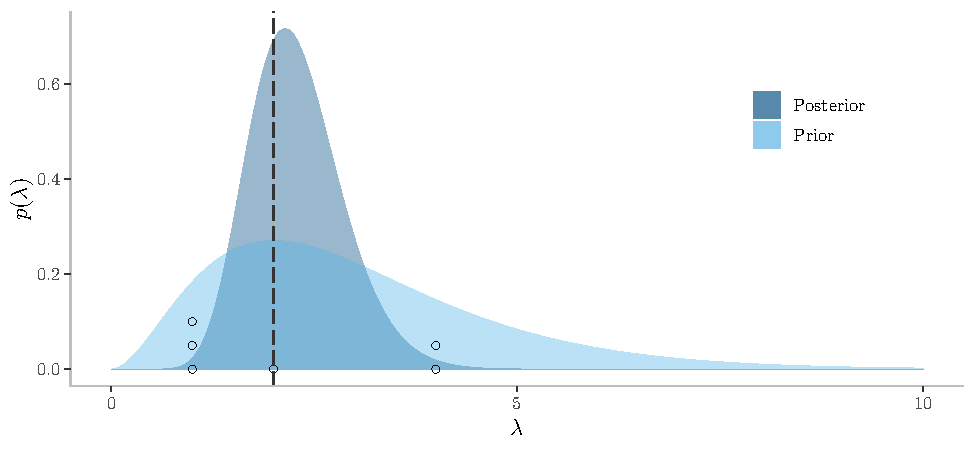
\includegraphics{thesis_files/figure-latex/unnamed-chunk-2-1.pdf}
\caption{\label{fig:unnamed-chunk-2}Particular example of Bayesian inference
for the Poisson-Gamma model. The prior hyperparameters are \(a = 3\) and
\(b = 1\). Data, plotted as open circles, is simulated from a Poisson
distribution with \(\lambda = 2\) shown as the dashed line.
\label{fig:bayes}}
\end{figure}

\section{\texorpdfstring{Graphical models
\label{sec:graph}}{Graphical models }}\label{graphical-models}

\begin{figure}
\centering
\begin{tikzpicture}[
      > = stealth, % arrow head style
      shorten > = 1pt, % don't touch arrow head to node
      auto,
      node distance = 3cm, % distance between nodes
      semithick % line style
    ]

    \node[] at (0, 1.5) {(a)};
    \node[state] (1) at (0, 0) {$Z_1$};
    \node[state] (2) at (2, 0) {$Z_2$};
    \node[state] (3) at (4, 0) {$Z_3$};
    \node[state] (4) at (6, 0) {$Z_4$};

    \path (1) edge (2);
    \path (2) edge (3);
    \path (3) edge (4);
    \path (1) edge[bend right=30] node [left] {} (3);
    \path (1) edge[bend right=50] node [left] {} (4);
    \path (2) edge[out=40, in=140]  (4);

    \node[] at (8, 1.5) {(b)};
    \node[state] (5) at (9, 1) {$Z_1$};
    \node[state] (6) at (11, 1) {$Z_2$};
    \node[state] (7) at (13, 1) {$Z_3$};
    \node[state] (8) at (11, -1) {$Z_4$};

    \path (5) edge (8);
    \path (6) edge (8);
    \path (7) edge (8);
\end{tikzpicture}
\caption{Directed acyclic graphs for the four variables $Z_1, \ldots, Z_4$.}
\label{fig:dag1}
\end{figure}

The particular features of the joint distribution \(p(\theta, Y)\) can
be constructed in many ways. Note that typically both \(\theta\) and
\(Y\) are multivariate, so specifying \(p(\theta, Y)\) may be no small
task. Probabilistic graphical models (PGMs) (Bishop
\protect\hyperlink{ref-bishop2006pattern}{2006}) are one popular and
useful tool for this purpose.

A graph \(\mathcal{G} = (\mathcal{V}, \mathcal{E})\) is defined by a set
of vertices \(\mathcal{V}\) together with a set of edges
\(\mathcal{E}\), where each edge connects a pair of vertices. In a PGM,
the vertices represent random variables and the edges represent
probabilistic relationships between the random variables. Bayesian
networks are a particular type of PGM in which conditional dependencies
(defined below) are the probabilistic relationships represented by the
edges (Bishop \protect\hyperlink{ref-bishop2006pattern}{2006}).

Consider random variables \(Z_k \in \mathcal{Z}_k\),
\(k = 1, \ldots, K\) with joint distribution \(p(Z_1, \ldots, Z_K)\).
\(Z_k\) is conditionally independent from \(Z_l\) given \(Z_m\), written
\(Z_k \perp Z_l \, | \, Z_m\), if and only if

\begin{equation}
p(Z_k, Z_l \, | \, Z_k) = p(Z_k \, | \, Z_k)p(Z_l \, | \, Z_k) \label{eq:cindepdef}
\end{equation}

By repeated conditioning, it is always true that the joint distribution
\(p(Z_1, \ldots, Z_K)\) can be decomposed according to

\begin{align}
p(Z_1, \ldots, Z_K) &= p(Z_1)p(Z_2, \ldots, Z_K \, | \, Z_1) = p(Z_1) p(Z_2 \, | \, Z_1) p(Z_3, \ldots, Z_K \, | \, Z_1, Z_2) \nonumber \\
&= \cdots = p(Z_1) p(Z_2 \, | \, Z_1) \cdots p(Z_K \, | \, Z_1, \ldots, Z_{K-1}). \label{eq:dag1}
\end{align}

This factorisation can be represented by a particular kind of graph
where the edges are directional, shown using arrows, and there are no
directed cycles between the nodes. Graphs like this are called directed
acyclic graphs (DAGs). A Bayesian network is a DAG where there is a
directed edge from variable \(Z_k\) to \(Z_l\) if the conditional
distribution of \(Z_l\) depends on \(Z_k\). For example, the DAG
corresponding to Equation \eqref{eq:dag1} with \(K = 4\) is shown in
part (a) of Figure \ref{fig:dag1}.

If Equation \eqref{eq:cindepdef} holds then conditional densities of the
form \(p(Z_k \, | \, Z_l, Z_k)\) can be rewritten to remove the
dependence on \(Z_l\) as follows

\begin{equation}
p(Z_k \, | \, Z_l, Z_k) = \frac{p(Z_k, Z_l \, | \, Z_k)}{p(Z_l \, | \, Z_k)} 
= \frac{p(Z_k \, | \, Z_k)p(Z_l \, | \, Z_k)}{p(Z_l \, | \, Z_k)}
= p(Z_k \, | \, Z_k). \label{eq:drop}
\end{equation}

Equation \eqref{eq:drop} shows that conditional independence statements
allow some of the dependencies, and hence directed edges in DAGs, to be
removed. Suppose that \(K = 4\) as before and each \(Z_1, Z_2\) and
\(Z_3\) are conditionally independent from each other given \(Z_4\).
Then, Equation \eqref{eq:dag1} may be rewritten as

\begin{equation}
p(Z_1, \ldots, Z_K) = p(Z_1)p(Z_2)p(Z_3)p(Z_4 \, | \, Z_1, Z_2, Z_3),  \label{eq:dag2}
\end{equation}

and the corresponding DAG redrawn taking into account this structure
(part (b) of Figure \ref{fig:dag1}).

It is visually clear that conditional independence statements result in
sparser graphs, thereby reducing model complexity. More generally, given
a set of conditional independence statements, joint probability
distributions may be rewritten as

\begin{equation}
p(Z_1, \ldots, Z_K) = \prod_{k=1}^K p(Z_k \, | \, \text{pa}(Z_k)),
\end{equation}

where \(Z_k\) is only conditionally dependent only on its parents
\(\text{pa}(Z_k)\). In the corresponding DAG, there is a directed edge
from each \(Z_l \in \text{pa}(Z_k)\) to \(Z_k\). For example, in Figure
\ref{fig:dag1}, \(\text{pa}(Z_4) = \{Z_1, Z_2, Z_3\}\).

Bayesian networks allow complex models \(p(Z_1, \ldots, Z_k)\) to be
built up from the simpler building blocks of
\(p(Z_k \, | \, \text{pa}(Z_k))\). In the context of Bayesian
statistics, supposing the prior parameter is multivariate
\(\theta = (\theta_1, \ldots, \theta_K)\) then the prior distribution
may be decomposed according to
\(\prod_{k=1}^K p(\theta_k \, | \, \text{pa}(\theta_k))\). The
statistical model \(p(\theta, Y)\) may then be written as a product of
the prior with the likelihood \(p(Y \, | \, \text{pa}(Y))\). Bayesian
models which are built up in stages this way are known as hierarchical
models.

These models possess the flexibility required to model the varied data
sources necessary for evidence synthesis. Furthermore, domain experts
can often efficaciously express their beliefs via Bayesian networks due
to their ease of interpretability.

\section{Modular models}\label{modular-models}

Having introduced the necessary prerequisites, we may now discuss how
they might be used to synthesise evidence.

Consider multiple sources of observable data \(Y_m \in \mathcal{Y}_m\)
with \(m = 1, \ldots M\). Each \(Y_m\) is, at least to some extent,
directly informative about a shared parameter \(\phi\) which is common
to all of the models. Therefore, for each evidence source, define a
statistical model \(p_m(\phi, \psi_m, Y_m)\), which will be henceforth
called a submodel. For each submodel the parameters are
\((\phi, \psi_m)\): the link parameter \(\phi \in \Phi\) together with
model specific parameters \(\psi_m \in \Psi_m\) unique to each submodel.

It is essential that each of the submodels agree conceptually on what
the link parameter \(\phi\) represents: conversations in which the
participants do not agree on the basic tenants are rarely productive. It
is worth mentioning this fact because in some models the interpretation
of parameters can be subtle. For example, in a regression the regression
coefficient of a covariate implicitly takes into account the inclusion
and exclusion of all other potential covariates; thereby making it a
different parameter in different models and rarely an appropriate link
parameter. It is therefore safest if \(\phi\) has a clear interpretation
linked to the real world.

Given the collection of submodels \(p_m(\phi, \psi_m, Y_m)\), the aim of
the joining operation in Markov melding (Goudie et al.
\protect\hyperlink{ref-goudie2019joining}{2019}) is to produce a joint
distribution \(p(\phi, \psi_1, \ldots, \psi_M, Y_1, \ldots, Y_M)\) over
all parameters and observable data. Synthesising a joint distribution is
attractive as it facilitates the propagation of uncertainty between the
submodels. Additionally, the joint distribution defines a statistical
model to which general methodological tools can be applied. Higher
quality inference about \(\phi\) is typically the primary aim of
evidence synthesis, although due to the sharing of information between
the submodels it may be that inference for \(\psi_m\)
\(m = 1, \ldots, M\) is also improved.

The joining of submodels is best suited to situations where the model
specific observed quantities \(Y_m\) are relatively distinct. The more
unique information there is dispersed across the different submodels,
the greater the potential benefits of evidence synthesis. On the other
extreme, the observed data \(Y_m = Y\) may be identical for each of the
\(M\) submodels (with different likelihood components say). This is in
some sense unappealing as each of the submodels then offers a competing
explanation for the data generating mechanism. Such a collection of
beliefs cannot be reasonably held confidently by a single individual
simultaneously. Rather, the individual may have to assign prior
probabilities to each of the models being true. Then, if the link
parameter plays different roles in the different submodels, although
Markov melding may be possible it might not be advisable. In machine
learning, multiple models may be trained on the same data and aggregated
for the purposes of prediction (Bishop
\protect\hyperlink{ref-bishop2006pattern}{2006}). However, in this
setting the focus is not on model building, interpretation or
uncertainty quantification.

Markov melding extends and unifies previous work, particularly Markov
combination (Dawid and Lauritzen
\protect\hyperlink{ref-dawid1993hyper}{1993}) and Bayesian melding
(Poole and Raftery \protect\hyperlink{ref-poole2000inference}{2000})
which we review here. In particular, Markov combination considers
joining submodels where an added simplifying assumption is made; whilst
Bayesian melding provides the methodological inspiration for overcoming
this assumption.

\section{Markov combination}\label{markov-combination}

As above consider the collection of submodels
\(p_m(\phi, \psi_m, Y_m)\), \(m = 1, \ldots, M\). Each submodel features
a prior distribution on the link parameter \(\phi\) which in the
simplest case is specified directly with
\(p_m(\phi, \psi_m, Y_m) = p_m(\psi_m, Y_m \, | \, \phi)p_m(\phi)\) such
that \(\text{pa}(\phi) = \emptyset\). Alternatively, the prior can be
accessed by marginalising out both \(\psi_m\) and \(Y_m\) as follows

\begin{equation}
p_m(\phi) = \iint p_m(\phi, \psi_m, Y_m) d\psi_m dY_m. \label{eq:priormarginal}
\end{equation}

An important property of the prior distributions is consistency; where
the marginals \(p_m(\phi)\) of the link parameter \(\phi\) are called
consistent if

\begin{equation}
\forall m \; p_m(\phi) = p(\phi). \label{eq:consistent}
\end{equation}

If the prior marginals are consistent then the submodels each have the
same beliefs about \(\phi\) in advance of seeing the data. As a result,
all of the submodels and their associated beliefs could theoretically
reasonably be held by a single individual without any
self-contradiction. (That being said, in practice a single practitioner
may justifiably place different priors on the same parameter depending
on the particular likelihood component. This might be the case if there
exists a conjugate prior, as in Example 2.1, for example.)

Supposing that assumption \eqref{eq:consistent} holds, Dawid and
Lauritzen (\protect\hyperlink{ref-dawid1993hyper}{1993}) define a joint
model
\(p_{\mathrm{comb}}(\phi, \psi_1, \ldots, \psi_M, Y_1, \ldots, Y_M)\)
called the Markov combination of the submodels \(p_1, \ldots, p_M\). In
advance of justification, this joint model \(p_{\mathrm{comb}}\) is

\begin{equation}
p_{\mathrm{comb}}(\phi, \psi_1, \ldots, \psi_M, Y_1, \ldots, Y_M) 
= \frac{\prod_{m=1}^{M} p_m(\phi, \psi_m, Y_m)}{p(\phi)^{M-1}}. \label{eq:comb}
\end{equation}

The construction of \(p_{\mathrm{comb}}\) is based on prior consistency
together with an additional assumption. This assumption is that,
conditional on the link parameter, the models are independent. To be
exact

\begin{equation}
\forall m \neq \ell \; (\psi_m, Y_m) \perp (\psi_\ell, Y_\ell) \, | \, \phi, \label{eq:cindep} 
\end{equation}

where conditional independence is defined as in Equation
\eqref{eq:cindepdef}. Figure \eqref{fig:cindepdag} illustrates this
assumption using a DAG for \(M = 2\) submodels.

In some sense, the truth of this assumption justifies the use of
seperate submodels, rather than a single monolithic model which is
specified at the outset. Just as with DAGs, conditional independence
statements simplify the process of modelling: it is easier to specify a
collection of submodels than it is to additionally consider their
interactions. This is particularly pertinent if the observable data
\(Y_m\) are from different background areas. Here, the modelling process
naturally decomposes such that different domain experts are consultated
for each data source, resuling in submodel specifications. In this
situation, the conditional independence assumption also seems, in
general, quite reasonable.

\begin{figure}
\centering
\begin{tikzpicture}[
      > = stealth, % arrow head style
      shorten > = 1pt, % don't touch arrow head to node
      auto,
      node distance = 3cm, % distance between nodes
      semithick % line style
    ]

    \node[state] (1) at (0,0){$\psi_1$};
    \node[state] (2) at (1,-2) {$Y_1$};
    \node[state] (3) at (2,0) {$\phi$};
    \node[state] (4) at (3,-2) {$Y_2$};
    \node[state] (5) at (4,0){$\psi_2$};

    \path (1) edge  (2);
    \path (3) edge  (2);
    \path (3) edge  (4);
    \path (5) edge (4);
\end{tikzpicture}
\caption{Directed acyclic graph corresponding to Equation \eqref{eq:cindep} for $M = 2$.}
\label{fig:cindepdag}
\end{figure}

The structure of Equation \eqref{eq:comb} is then explained by applying
these two assumptions to a hypothetical joint model

\begin{align}
p(\phi, \psi_1, \ldots, \psi_M, Y_1, \ldots, Y_M)
&\stackrel{\phantom{\eqref{eq:cindep}}}{=} p(\phi) \, p(\psi_1, \ldots, \psi_M, Y_1, \ldots, Y_M \, | \, \phi) \nonumber \\
&\stackrel{\eqref{eq:cindep}}{=} p(\phi) \prod_{m=1}^{M} p_m(\psi_m, Y_m \, | \, \phi) \nonumber \\
&\stackrel{\phantom{\eqref{eq:cindep}}}{=} p(\phi) \prod_{m=1}^M \frac{p_m(\phi, \psi_m, Y_m)}{p_m(\phi)} \label{eq:premeld} \\
&\stackrel{\eqref{eq:consistent}}{=} \frac{\prod_{m=1}^{M} p_m(\phi, \psi_m, Y_m)}{p(\phi)^{M-1}},
\end{align}

where the result is exactly that of Equation \eqref{eq:comb}.

Markov combination has the attractive property that submodel marginals
and submodel-specific conditional distributions are preserved, that is
\(p_{\mathrm{comb}}(\phi, \psi_m, Y_m) = p_m(\phi, \psi_m, Y_m)\) and
\(p_{\mathrm{comb}}(\psi_m, Y_m \, | \, \phi) = p_m(\psi_m, Y_m \, | \, \phi)\)
for all \(m\) (Goudie et al.
\protect\hyperlink{ref-goudie2019joining}{2019}). This can be shown via

\begin{align}
p_{\mathrm{comb}}(\phi, \psi_m, Y_m) &= \int p_{\mathrm{comb}}(\phi, \psi_1, \ldots, \psi_M, Y_1, \ldots, Y_M) d\psi_{-m} dY_{-m} \nonumber \\
&= \int p(\phi) \prod_{m=1}^{M} p_m(\psi_m, Y_m \, | \, \phi) d\psi_{-m} dY_{-m} \nonumber \\
&= p(\phi) p_m(\psi_m, Y_m \, | \, \phi) = p_m(\phi, \psi_m, Y_m),
\end{align}

where the notation \(d\psi_{-m} dY_{-m}\) refers to integration with
respect to each of the model specific parameters and observed quantites
except from \(\psi_m\) and \(Y_m\). Similarly

\begin{align}
p_{\mathrm{comb}}(\psi_m, Y_m \, | \, \phi) &= \frac{p_{\mathrm{comb}}(\phi, \psi_m, Y_m)}{p(\phi)} = \frac{p(\phi, \psi_m, Y_m)}{p(\phi)} = p_m(\psi_m, Y_m \, | \, \phi).
\end{align}

In its form, the Markov melded joint model is similar to that of Markov
combination. This is because both methods assume the conditional
independence assumption, given by Equation \eqref{eq:cindep}. The
primary difference is that Markov melding does not assume that the prior
marginals of the link parameter are consistent. Instead, these marginals
are ``melded'' by a process similar to that developed in Bayesian
melding, which we will now detail.

\section{\texorpdfstring{Bayesian melding
\label{sec:bayesianmelding}}{Bayesian melding }}\label{bayesian-melding}

The presence of multiple priors on a given quantity also arises in the
study of simulation models. Bayesian melding (Poole and Raftery
\protect\hyperlink{ref-poole2000inference}{2000}) is motivated by this
challenge and aims to perform inference on deterministic simulation
models \(M: \theta \to \phi\). The outputs
\(\phi \in \Phi \subseteq \mathbb{R}^p\) are a function of the inputs
\(\theta \in \Theta \subseteq \mathbb{R}^n\) only, such that
\(\phi = M(\theta)\). There may exist data relating to one or both of
\(\theta\) and \(\phi\) which we denote by \(Y_\theta\) and \(Y_\phi\)
respectively. Irrespective of the simulation model \(M\), a statistical
model \(p(\theta, \phi, Y_\theta, Y_\phi)\) can be specified which Poole
and Raftery (\protect\hyperlink{ref-poole2000inference}{2000})
additionally assume can be decomposed into a product of independent
prior and likelihood components

\begin{equation}
p(\theta, \phi, Y_\theta, Y_\phi) = p(Y_\theta \, | \, \theta)p(\theta)p(Y_\phi \, | \, \phi)p(\phi).
\end{equation}

We call this distribution the joint premodel prior distribution. It may
be marginalised to find the premodel prior distributions \(p(\theta)\)
and \(p(\phi)\) respectively.

Bayesian melding builds upon a previous approach called Bayesian
synthesis (Raftery, Givens, and Zeh
\protect\hyperlink{ref-raftery1995inference}{1995}). In this approach,
the model \(M\) is incorporated into the joint premodel distribution to
create a joint postmodel distribution
\(\pi(\theta, \phi, Y_\theta, Y_\phi)\). Poole and Raftery
(\protect\hyperlink{ref-poole2000inference}{2000}) describe that this is
done by restricting \(p(\theta, \phi, Y_\theta, Y_\phi)\) to the
submanifold \(\{(\theta, \phi, Y_\theta, Y_\phi):\phi = M(\theta)\}\),
such that

\begin{equation}
\pi(\theta, \phi, Y_\theta, Y_\phi) \propto
\begin{cases}
  p(\theta, M(\theta), Y_\theta, Y_\phi), & \text{if } \phi = M(\theta) \\
  0, & \text{otherwise.}
\end{cases}
\end{equation}

The marginal postmodel prior distribution for \(\theta\) is then

\begin{equation}
\pi(\theta) = p(\theta \, | \, \phi = M(\theta)) \label{eq:wolpert}
\end{equation}

However, in a discussion of the paper, Wolpert
(\protect\hyperlink{ref-wolpert1995inference}{1995}) call attention to
the fact that conditional distributions of the form \eqref{eq:wolpert}
are ill-defined and therefore subject to what is known as the
Borel-Kolmogorov paradox. A key repercussion of this fact is that the
postmodel distribution depends on how \(M\) is parametrised.
Furthermore, Schweder and Hjort
(\protect\hyperlink{ref-schweder1996bayesian}{1996}) show that any
postmodel distribution can be obtained by arbitrary parametrisation of
\(M\). These observations place serious concern on the usefulness of
Bayesian synthesis, motivating the development of Bayesian melding.

The problem that Wolpert
(\protect\hyperlink{ref-wolpert1995inference}{1995}) find arises because
in Bayesian synthesis, as well as the premodel marginal prior
distribution \(p(\phi)\), there is an additional prior on the output
\(\phi\). In particular, applying the deterministic model \(M\) to the
premodel marginal prior distribution on inputs \(p(\theta)\) results in
a model-induced prior on outputs \(\phi\) denoted by \(p^\star(\phi)\).
If \(M^{-1}\) exists then this prior is given by

\begin{equation}
p^\star(\phi) = p(M^{-1}(\phi)) |J(\phi)|, \label{eq:transform}
\end{equation}

where \(J(\phi)\) is the Jacobian of the transformation. The two priors
are typically inconsistent as they are based on different information.

A simple approach to rectifying this problem would be not to attempt to
place a separate prior on outputs \(\phi\), instead relying on the prior
induced by applying \(M\) to \(p(\theta)\) However, in hopes of
combining both information from the premodel prior and that of the model
induced prior, Bayesian melding instead replaces \(p(\phi)\) and
\(p^\star(\phi)\) by a single melded output prior \(\tilde p(\phi)\).
For their particular motivating application, relating to a population
dynamics model for bowhead whales, Poole and Raftery
(\protect\hyperlink{ref-poole2000inference}{2000}) do this by taking the
(normalised) geometric mean of the two priors as follows

\begin{equation}
\tilde p(\phi) \propto p(\phi)^{0.5}p^\star(\phi)^{0.5} \label{eq:geometric}
\end{equation}

Equation \eqref{eq:geometric} is an example of a broader class of
pooling operations which mathematically combine probability
distributions. More examples will be discussed further in the next
section.

Poole and Raftery (\protect\hyperlink{ref-poole2000inference}{2000})
propose then inverting the prior \(\tilde p(\phi)\) to the input space
to define a melded input prior \(\tilde p(\theta)\) as (omitting some
details)

\begin{align}
\tilde p(\theta) &= \tilde p(M(\theta)) \left(\frac{p(\theta)}{p^\star(M(\theta))}\right) \nonumber \\
&\propto p(\theta) \left(\frac{p(M(\theta))}{p^\star(M(\theta))}\right)^{1-\alpha}. \label{eq:inversion}
\end{align}

Equation \eqref{eq:inversion} corresponds to the original input prior
\(p(\theta)\) weighted, according to \(\alpha\), by a ratio of the
output prior and the model induced prior evaluated at
\(\phi = M(\theta)\) for given value of \(\theta \in \Theta\).

To conclude discussion of Bayesian melding, having observed
\(Y_\theta = y_\theta\) and \(Y_\phi = y_\phi\) a standard Bayesian
posterior for \(\theta\) can be then defined as follows

\begin{equation}
\pi(\theta \, | \, y_\phi, y_\theta) \propto p(y_\theta \, | \, \theta)p(y_\phi \, | \, M(\theta)) \tilde p(\theta),
\end{equation}

allowing inference to proceed as usual.

\section{\texorpdfstring{Combining expert opinion
\label{sec:experts}}{Combining expert opinion }}\label{combining-expert-opinion}

The prior pooling step, for which Equation \eqref{eq:geometric} is one
instance, in Bayesian melding has methodological similarities with
previous work on combining the opinions of multiple experts (O'Hagan et
al. \protect\hyperlink{ref-o2006uncertain}{2006}). Most relevant from
this literature is mathematical aggregation, where distributions are
elicited independently from each expert individually and then combined
by some mathematical rule. The primary alternative to mathematical
aggregation is behavioural aggregation, where the group of experts
interact and a single distribution is elicited from the group after
discussion. In the case of Markov melding, in general the practitioners
who originally developed each of the submodels may not be willing and
able to justify their choices as would be required in behavioural
aggregation.

Just as it is important that the submodels in Markov melding have a
shared concept of the link parameter, Clemen and Winkler
(\protect\hyperlink{ref-clemen1999combining}{1999}) caution that ``the
mathematical and behavioural approaches \ldots{} assume that the experts
have ironed out differences in definitions and that they agree on
exactly what is to be forecast or assessed''; also noting that
``practising risk analysts know these are strong assumptions''.

In order to outline some of the proposed (O'Hagan et al.
\protect\hyperlink{ref-o2006uncertain}{2006}) approaches, suppose each
of a group of \(n\) experts are independently asked their beliefs about
an unknown quantity \(\theta\), resulting in elicited distributions
\(f_i(\theta), i = 1, \ldots, n\). The simplest and most widely used
technique within mathematical aggregation is opinion pooling, where a
consensus distribution \(f(\theta)\) is obtained as some function of the
individual distributions \(\{f_1(\theta), \ldots, f_n(\theta)\}\). Two
of the most common examples are the linear opinion pool
\eqref{eq:linpool} and logarithmic opinion pool \eqref{eq:logpool}
defined respectively as

\begin{align}
f(\theta) \propto \sum_{i=1}^{n} w_i f_i(\theta) \label{eq:linpool}, \\ 
f(\theta) \propto \prod_{i=1}^{n} f_i(\theta)^{w_i} \label{eq:logpool},
\end{align}

where \(f(\theta)\) is normalised to a probability density function. The
weights \(w_i\) can be chosen freely, either giving more weight to some
experts than others or choosing to weight all of the experts equally.

Dictatorial pooling, in which one experts opinion is chosen as the
consensus distribution, is special case of linear opinion pooling. To
see this, set \(w_j = 0\) for all \(j \neq i\) in Equation
\eqref{eq:linpool} such that \(f(\theta) = f_i(\theta)\). In Section
\ref{sec:bayesianmelding}, the suggestion to set
\(\tilde p(\phi) = p^\star(\phi)\) is an example of dictatorial pooling.
The method used by Poole and Raftery
(\protect\hyperlink{ref-poole2000inference}{2000}), geometric pooling
given by Equation \eqref{eq:geometric}, is an example of logarithmic
pooling with \(w_i = 1/M\). Another special case of logarithmic opinion
pooling is the product of experts pooling (Hinton
\protect\hyperlink{ref-hinton2002training}{2002}) which sets \(w_i = 1\)
for all \(i\) such that

\begin{equation}
f(\theta) \propto \prod_{i=1}^{n} f_i(\theta). \label{eq:poe}
\end{equation}

\begin{figure}
\centering
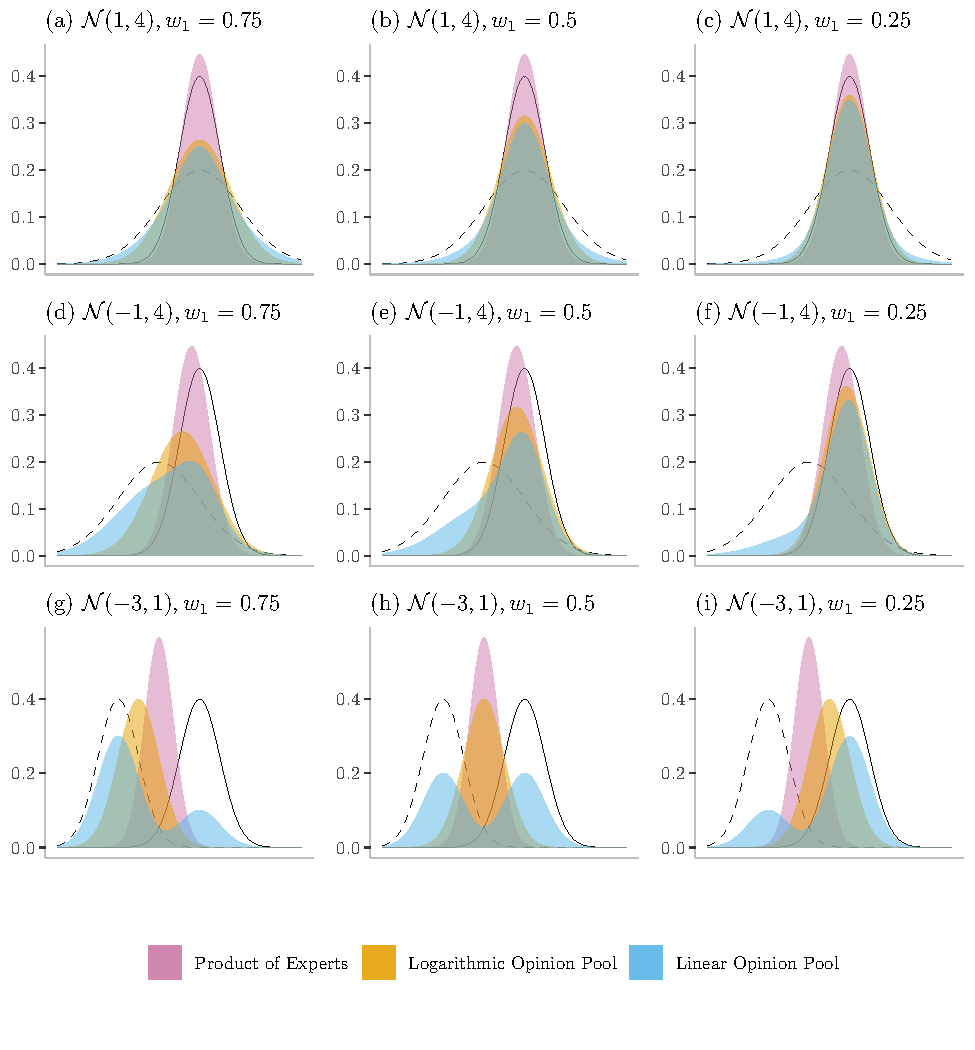
\includegraphics{thesis_files/figure-latex/unnamed-chunk-3-1.pdf}
\caption{\label{fig:unnamed-chunk-3}Opinion pooling of solid line
\(\mathcal{N}(1, 1)\) with dashed line Gaussians, specified by plot
text. Dashed line Gaussians are weighted \(w_1\) with \(w_2 = 1 - w_1\).
Reproduced with alternations from Goudie et al.
(\protect\hyperlink{ref-goudie2019joining}{2019}). \label{fig:pooling}}
\end{figure}

Figure \eqref{fig:pooling} shows the Product of Experts, logarithmic and
linear opinion pooling applied to various Gaussian distributions. Note
that in the Product of Experts pooling, there are no weights. Or,
another way of looking at it, the weights are fixed to be
\(w_1 = w_2 = 1\).

The Product of Experts is named as such because it gives each expert the
benefit of the doubt in assuming that their beliefs are correct. The
result, as most clearly illustrated by row (g, h, i) of Figure
\eqref{fig:pooling}, is that the regions where the experts overlap has
to be the truth. Logarithmic pooling is slightly more doubtful of the
experts but still produces relatively contracted pooled beliefs in
comparison to the more cautious linear pooling. O'Hagan et al.
(\protect\hyperlink{ref-o2006uncertain}{2006}) find that ``while the
linear opinion pool has been quite widely used in practice, the
logarithmic opinion pool has been largely ignored, perhaps because it is
perceived to lead to unrealistically strong aggregated beliefs''.

Row (a, b, c) of Figure \eqref{fig:pooling} prompt another
consideration: to what extend should expert agreement lead to higher
confidence. To use an analogy, suppose you and a group of friends want
to decide whether or not to eat at a certain restaurant. If each friend
expresses a positive opinion about the restaurant then may seem
reasonable to be more confident than any given friend about the
restaurant. However, if each friend bases their opinion solely on a
positive review of the restaurant in that week's paper then this
effectively would be double counting; in reality there is only one
``expert'' - the journalist.

\section{Markov melding}\label{markov-melding}

If the marginals are inconsistent, that is condition
\eqref{eq:consistent} fails to hold, then the approach of Markov
combination requires some modification. Just as pooling is used to
reconcile disagreement between the premodel prior and induced prior in
Bayesian melding, the inconsistent prior marginals \(p_m(\phi)\) can be
also pooled to allow Bayesian inference to proceed. The resulting pooled
prior \(p_\text{pool}(\phi)\) is such that

\begin{equation}
p_\text{pool}(\phi) = g(p_1(\phi), \ldots, p_M(\phi)), \label{eq:pooledprior}
\end{equation}

for some choice of pooling function \(g\). As discussed in Section
\ref{sec:experts}, many possible pooling functions are possible and
could be reasonably justified depending on the situation. That being
said, some choices of pooling function may be more computational
efficient and so attractive from a practical point of view.

The Markov melded joint model \(p_{\text{meld}}\) can be achieved by
replacing \(p(\theta)\) in Equation \eqref{eq:premeld} with the pooled
prior \eqref{eq:pooledprior} such that

\begin{equation}
p_{\text{meld}}(\phi, \psi_1, \ldots, \psi_M, Y_1, \ldots, Y_M) = p_\text{pool}(\phi) \prod_{m=1}^M \frac{p_m(\phi, \psi_m, Y_m)}{p_m(\phi)} \label{eq:meld}
\end{equation}

This construction is equivalent to altering each of the submodels by a
procedure Goudie et al.
(\protect\hyperlink{ref-goudie2019joining}{2019}) call marginal
replacement and then applying Markov combination. In particular, the
marginal \(p_m(\phi)\) of the original submodel is replaced by
\(p_\text{pool}(\phi)\) resulting in the replacement submodel

\begin{equation}
p_{\text{repl,m}}(\phi, \psi_m, Y_m) = p_m(\psi_m, Y_m \, | \, \phi)p_\text{pool}(\phi).
\end{equation}

After marginal replacement has occurred it is possible to apply Markov
combination to the collection of replacement submodels
\(\{p_{\text{repl,m}}\}_{m = 1,\ldots,M}\) since they have consistent
marginals, such that

\begin{align}
p_{\mathrm{comb}}(\phi, \psi_1, \ldots, \psi_M, Y_1, \ldots, Y_M) 
&= \frac{\prod_{m=1}^{M} p_{\text{repl,m}}(\phi, \psi_m, Y_m)}{p_\text{pool}(\phi)^{M-1}} \nonumber \\
&= \frac{\prod_{m=1}^{M} p_m(\psi_m, Y_m \, | \, \phi)p_\text{pool}(\phi)}{p_\text{pool}(\phi)^{M-1}} \nonumber \\
&= p_\text{pool}(\phi) \prod_{m=1}^{M} p_m(\psi_m, Y_m \, | \, \phi) \nonumber \\
&= p_\text{pool}(\phi) \prod_{m=1}^{M} \frac{p_m(\psi_m, Y_m, \phi)}{p_m(\phi)}.
\end{align}

The result is equal to that of the Markov melded joint model, Equation
\eqref{eq:meld}.

Since a joint model has been obtained, Bayesian inference can proceed as
usual. Given observed data \(Y_m = y_m\) for \(m = 1, \ldots, M\), under
the Markov melded model \eqref{eq:meld} the joint posterior distribution
is

\begin{align}
p_{\text{meld}}(\phi, \psi_1, \ldots, \psi_M \, | \, y_1, \ldots, y_M) \propto p_{\text{pool}}(\phi) \prod_{m=1}^{M} \frac{p_m(\phi, \psi_m, y_m)}{p_m(\phi)}, \label{eq:meldpost}
\end{align}

which is called the Markov melded posterior.

We present the following pedagogical example of Markov melding with
\(M = 2\) submodels which, as with Example 3.1, uses conjugacy to enable
exact Bayesian computation.

\emph{Example 2.2: Binomial and Geometric submodels with conjugate Beta
priors}

\begin{figure}
\centering
\begin{tikzpicture}[
      > = stealth, % arrow head style
      shorten > = 1pt, % don't touch arrow head to node
      auto,
      node distance = 3cm, % distance between nodes
      semithick % line style
    ]

    \node[] at (0, 1) {(a) Submodel 1: $p_1(\theta, Y_1)$};
    \node[constant] (1) at (0,0){$a$};
    \node[constant] (2) at (2,0) {$b$};
    \node[state] (3) at (1,-2) {$\theta$};
    \node[constant] (4) at (3,-2) {$m$};
    \node[state] (5) at (2,-4){$Y_1^i$};
    \node[above right] at (0, -5) {$i = 1, \ldots, n_1$}; 

    \path (1) edge  (3);
    \path (2) edge  (3);
    \path (3) edge  (5);
    \path (4) edge (5);
    
    \draw (0,-3) -- (3,-3) -- (3,-5) -- (0,-5) -- cycle;

    \node[] at (7, 1) {(b) Submodel 2: $p_2(\theta, Y_2)$};
    \node[constant] (6) at (7,0){$c$};
    \node[constant] (7) at (9,0) {$d$};
    \node[state] (8) at (8,-2) {$\theta$};
    \node[state] (9) at (8,-4) {$Y_2^i$};
    \node[above right] at (6.5,-5) {$i = 1, \ldots, n_2$}; 

    \path (6) edge  (8);
    \path (7) edge  (8);
    \path (8) edge  (9);
    
    \draw (6.5,-3) -- (9.5,-3) -- (9.5,-5) -- (6.5,-5) -- cycle;
    
\end{tikzpicture}
\caption{Further to the notation introduced in Section \ref{sec:graph}, constants may be included in DAGs with square boxes, whereas random variables have circular boxes. Rectangular boxes (sometimes called plates) are drawn around sections of the diagram which are repeated across the indices indicated.}
\label{fig:ex1dag}
\end{figure}

Consider the following two submodels, illustrated as DAGs in Figure
\ref{fig:ex1dag}.

\textbf{Submodel 1} Define the first submodel \(p_1(\theta, Y_1)\) as

\begin{align}
\theta &\sim \text{Beta}(a, b), \label{eq:prior1} \\
Y_1^i &\sim \text{Bin}(m, \theta), \quad i = 1, \ldots, n_1,
\end{align}

where \(a = 2\), \(b = 3\) and \(m = 10\) are known and
\(Y_1 = (Y_1^1, \ldots, Y_1^{n_1})\).

Suppose the true value of \(\theta = 0.4\). We simulate observed data
\(Y_1 = y_1\) and of size \(n_1 = 3\) from this submodel, resulting in
\(y_1 = \{3, 5, 4\}\). Conditioning on the observed data, inference can
be done exactly as the prior is conjugate. The posterior distribution is
given by

\begin{align}
p_1(\theta \, | \, y_1) &\propto p_1(y_1 \, | \, \theta) p_1(\theta) 
= \prod_{i=1}^{n_1} {m\choose y_1^i} \theta^{y_1^i}  (1- \theta)^{m-{y_1^i}} \cdot 
   \frac{\Gamma(a)\Gamma(b)}{\Gamma(a+b)} \theta^{a-1} (1- \theta)^{b-1} \nonumber \\
&\propto \theta^{\tau_1 + a - 1}  (1- \theta)^{n_1m-\tau_1 + b - 1} 
\propto \text{Beta}(\tau_1 + a, n_1m-\tau_1 + b),
\end{align}

where \(\sum_{i=1}^{n_1} y_1^i = \tau_1\).

\textbf{Submodel 2} The second submodel \(p_2(\theta, Y_2)\) is such
that

\begin{align}
\theta &\sim \text{Beta}(c, d) \label{eq:prior2} \\
Y_2 &\sim \text{Geo}(\theta), \quad i = 1, \ldots, n_2,
\end{align}

where \(c = 5\) and \(d = 4\) are known and
\(Y_1 = (Y_2^1, \ldots, Y_2^{n_2})\).

We again simulate observed data \(Y_2 = y_2\) this time of size
\(n_2 = 6\), resulting in \(y_2 = \{2, 0, 1, 0, 0, 1\}\). This submodel,
like the one before, is conjugate and the posterior distribution is
simply

\begin{align}
p_2(\theta \, | \, y_2) &\propto p_2(y_2 \, | \, \theta) p_2(\theta)
= \prod_{i=1}^{n_2} (1-\theta)^{y_2^i} \theta \cdot 
   \frac{\Gamma(c)\Gamma(d)}{\Gamma(c+d)} \theta^{c-1} (1- \theta)^{d-1} \nonumber \\
&\propto \theta^{n_2 + c - 1}  (1- \theta)^{\tau_2 + d - 1}
\propto \text{Beta}(n_2 + c, \tau_2 + d),
\end{align}

where \(\sum_{i=1}^{n_2} y_2^i = \tau_2\).

\begin{figure}
\centering
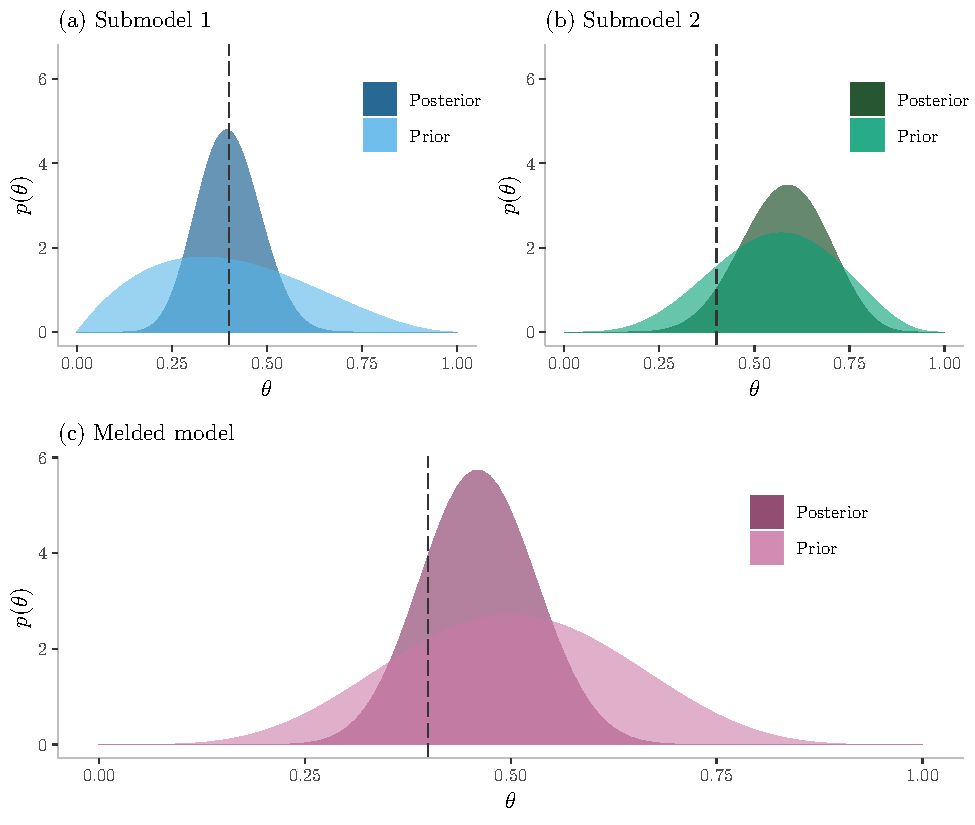
\includegraphics{thesis_files/figure-latex/unnamed-chunk-5-1.pdf}
\caption{\label{fig:unnamed-chunk-5}Parts (a) and (b) show the standard
Bayesian updating of the prior for submodels one and two respectively.
Part (c) shows the PoE pooled prior and Markov melded posterior.
\label{fig:ex1}}
\end{figure}

\textbf{Melded model} This is a simple situation: the link parameter is
\(\phi = \theta\), and there are no model specific parameters
\(\psi_1 = \psi_2 = \emptyset\). Notice with this hyperparameter
setting, there is not consistency between the two Beta priors, given by
Equations \eqref{eq:prior1} and \eqref{eq:prior2}, on the link
parameter. For this reason, Markov melding is an appropriate
methodological choice to perform inference.

To facilitate Markov melding, we pool the inconsistent prior
distributions \(p_1(\theta)\) and \(p_2(\theta)\). Using the Product of
Experts pooling \eqref{eq:poe} gives the pooled prior to be

\begin{align}
p_\text{pool}(\theta) &\propto \text{Beta}(a, b) \cdot \text{Beta}(c, d) 
                      \propto \theta^{a-1}(1 - \theta)^{b-1} \cdot \theta^{c-1}(1 - \theta)^{d-1} \nonumber \\
                      &= \theta^{a + c - 2}(1 - \theta)^{b + d - 2} \propto \text{Beta}(a + c - 1, b + d - 1). \label{eq:pooledbeta}
\end{align}

By Equation \eqref{eq:meldpost}, the relevant Markov melded posterior is

\begin{align}
p_{\text{meld}}(\theta \, | \, y_1, y_2)
&\propto p_{\text{pool}}(\theta) \prod_{m=1}^{2} \frac{p_m(\theta \, | \, y_m)}{p_m(\theta)}
\propto p_1(\theta)p_2(\theta) \prod_{m=1}^{2} \frac{p_m(\theta \, | \, y_m)}{p_m(\theta)} \nonumber \\
&\propto p_1(\theta \, | \, y_1)p_2(\theta \, | \, y_2) \nonumber \\
&\propto \text{Beta}(\tau_1 + a + n_2 + c - 1, n_1m-\tau_1 + b + \tau_2 + d - 1). \label{eq:meldedbeta}
\end{align}

In fact, in general under Product of Experts pooling, the melded
posterior is proportional to the product of the submodel posteriors

\begin{align}
p_{\text{meld}}(\phi, \psi_1, \ldots, \psi_M \, | \, y_1, \cdots, y_M) 
&\propto p_{\text{pool}}(\phi) \prod_{m=1}^{M} \frac{p_m(\phi, \psi_m, y_m)}{p_m(\phi)} \nonumber \\
&= \prod_{m=1}^{M} p_m(\phi, \psi_m, y_m) \nonumber \\
&\propto \prod_{m=1}^{M} p_m(\phi, \psi_m \, | \, y_m). \label{eq:poecancel}
\end{align}

Figure \ref{fig:ex1} shows that both the melded prior
\eqref{eq:pooledbeta} and Markov melded posterior \eqref{eq:meldedbeta}
occupy a centrist position between the two submodels.

Suppose rather than Product of Experts pooling we use logarithmic
pooling with weights \(w_m\) for submodel \(m\) such that
\(w_1 + w_2 = 1\). The pooled prior is then

\begin{align}
p_\text{pool}(\theta) &\propto \text{Beta}(a, b)^{w_1} \cdot \text{Beta}(c, d)^{w_2}
                      \propto \theta^{w_1(a-1)}(1 - \theta)^{w_1(b-1)} \cdot \theta^{w_2(c-1)}(1 - \theta)^{w_2(d-1)} \nonumber \\
                      &\propto \text{Beta}(w_1a + w_2c - w_1 - w_2 + 1, w_1b + w_2d - w_1 - w_2 + 1)
                      \propto \text{Beta}(e, f),
\end{align}

where \(e = w_1a + w_2c - w_1 - w_2 + 1\) and
\(f = w_1b + w_2d - w_1 - w_2 + 1\). Using this pooled prior, the Markov
melded posterior is given by

\begin{align}
p_{\text{meld}}(\theta \, | \, y_1, y_2)
&\propto p_{\text{pool}}(\theta) \prod_{m=1}^{2} \frac{p_m(\theta \, | \, y_m)}{p_m(\theta)} \nonumber \\
&\propto \text{Beta}(e, f) 
\frac{\text{Beta}(\tau_1 + a, n_1m-\tau_1 + b)}{\text{Beta}(a, b)} \frac{\text{Beta}(n_2 + c, \tau_2 + d)}{\text{Beta}(c, d)} \nonumber \\
&\propto \theta^{e + \tau_1 + n_2 - 1}
         (1 - \theta)^{f + n_1m - \tau_1 + \tau_2 - 1} \nonumber \\
&\propto \text{Beta}(e + \tau_1 + n_2, f + n_1m - \tau_1 + \tau_2)
\end{align}

Note that setting \(w_1 = w_2 = 1\) gives, as in Equation
\eqref{eq:meldedbeta}, a
\(\text{Beta}(a + c + \tau_1 + n_2 - 1, b + d + n_1m - \tau_1 + \tau_2 - 1)\)
distribution. Figure \ref{fig:ex1weight} shows the results of Markov
melding for three weight settings. In parts (a) and (c) the weighting
amounts to dictatorial pooling to submodels one and two respectively.
Part (b), in contrast, is a geometric mean between the two submodels.
Under these circumstances of the particular pooling is of little
consequence to the Markov melded posterior. \hfill \(\square\)

\begin{figure}
\centering
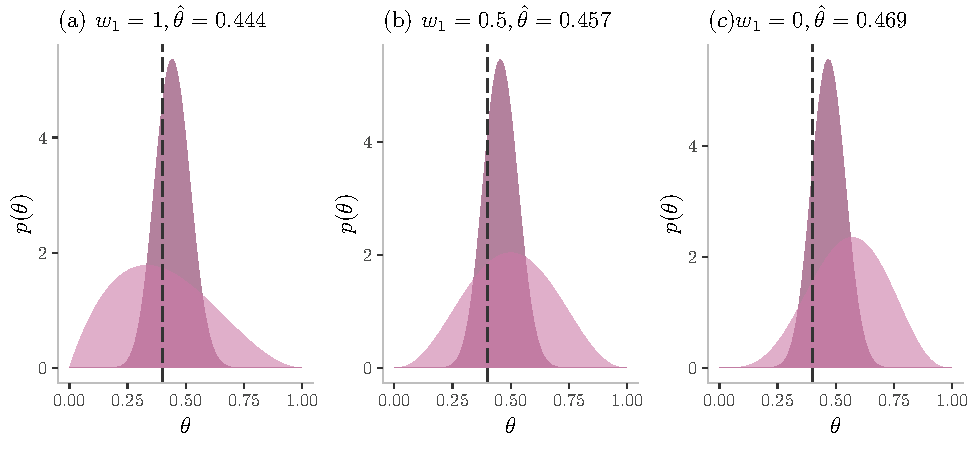
\includegraphics{thesis_files/figure-latex/unnamed-chunk-6-1.pdf}
\caption{\label{fig:unnamed-chunk-6}Markov melding using logarithmically
pooled priors with various weights. The weighting \(w_1\), with
\(w_2 = 1 - w_1\), as well as the posterior mean
\(\hat \theta = \mathbb{E}[\theta \, | \, y_1, y_2]\) is given above
each plot. \label{fig:ex1weight}}
\end{figure}

Example 2.2 shows that, for a simple tractable case, Markov melding
behaves as one would hope.

\chapter{\texorpdfstring{Computation
\label{chapter:comp}}{Computation }}\label{computation}

The primary goal in Bayesian computation is to find expectations of
functions with respect to the posterior distribution, or in our case the
Markov melded posterior given by Equation \eqref{eq:meldpost}. Many
relevant quantities, such as probabilities or risks, can be cast as
integrals as the following example demonstrates.

\emph{Example 3.1: Bayesian decision theory}

In assessing developments in evidence-based medicine, Ashby and Smith
(\protect\hyperlink{ref-ashby2000evidence}{2000}) argue that a Bayesian
approach is the natural framework for decision making under uncertainty.
Suppose \(\mathcal{A}\) is the space of possible decisions with elements
\(a \in \mathcal{A}\) and there exists a utility function
\(U: \mathcal{A} \to \mathbb{R}^+\) weighing up the drawbacks and
benefits of each decision. Then, it is clear to see that the optimal
decision is to select the decision \(a^\star\) which maximises this
utility. Leaving aside the problem of specifying \(U\), most (if not
all) of the time the utility also depends on additional variables which
we are uncertain about. If these additional variables are (leadingly)
denoted by \(\theta \in \Theta\) then our definition of \(U\) may be
expanded so that \(U: \mathcal{A} \times \Theta \to \mathbb{R}^+\). Now,
in order to make well-informed decisions, we must take into account our
uncertainty about \(\theta\). Having observed data \(y \in \mathcal{Y}\)
informative about \(\theta\), the distribution which represents this
uncertainty is the posterior \(p(\theta \, | \, y)\). Rather than
computing utilities, we now must calculate expected utilities. This is
done by integrating out our uncertainty about \(\theta\) as follows

\begin{equation}
\mathbb{E}_{p(\theta \, | \, y)}[U(a, \theta)] = \int U(a, \theta) p(\theta \, | \, y) d\theta. \label{eq:bayesdecision}
\end{equation}

The optimal decision now is to select the action maximising this
expected utility. The upshot is that Equation \eqref{eq:bayesdecision}
amounts to computing expectations with respect to the posterior.
\hfill \(\square\)

\section{Monte Carlo methods}\label{monte-carlo-methods}

Monte Carlo, a general class of simulation-based methods, are a
prevailing technique for scalable computation of integrals like that of
Equation \eqref{eq:bayesdecision}. For ease of notation rather than the
posterior, we consider a general probability density function \(\pi(x)\)
where \(x \in \mathcal{X}\). The relevant integral is then

\begin{equation}
\mathbb{E}_\pi[\varphi(x)] = \int \varphi(x) \pi(x) dx
\end{equation}

where \(\varphi: \mathcal{X} \to \mathbb{R}\) is an arbitrary test
function.

By sampling points independently from the probability density function
\(X_i \sim \pi(x)\) for \(i = 1,\ldots, N\), \(\pi(x)\) may be
approximated by the empirical distribution

\begin{equation}
\widehat{\pi}(x) = \frac{1}{N} \sum_{i=1}^{N} \delta_{X_i}(x). \label{eq:empirical}
\end{equation}

This facilitates the approximation of expectations by using
\(\widehat{\pi}(x)\) in place of \(\pi(x)\) such that

\begin{equation}
\mathbb{E}_\pi[\varphi(x)] = \int \varphi(x) \pi(x) dx \approx \int \varphi(x) \widehat{\pi}(x) dx = \frac{1}{N} \sum_{i=1}^{N} \varphi(X_i) := \bar \varphi_N. \label{eq:monte}
\end{equation}

By the strong law of large numbers, granted the expectation exists, then
the Monte Carlo estimator will converge

\begin{equation}
\lim_{N\to\infty} \bar \varphi_N = \mathbb{E}_\pi[\varphi(x)] 
\end{equation}

almost surely. In addition, the rate of convergence can be monitored by
estimating the variance of the Monte Carlo estimator \(\bar \varphi_N\)
as

\begin{equation}
\sigma^2_N = \frac{1}{N^2} \sum_{i=1}^{N} \left( \varphi(x_i) - \bar \varphi_N \right)^2,
\end{equation}

and then applying the central limit theorem such that

\begin{equation}
\frac{\bar \varphi_N - \mathbb{E}_\pi[\varphi(x)]}{\sigma_N} \sim \mathcal{N}(0, 1).
\end{equation}

These principles, both the approximation of the empirical distribution
via Equation \eqref{eq:empirical} and the convergence of the Monte Carlo
estimator, are illustrated in Figure \eqref{fig:monte} for a simple
exponential distribution with rate parameter \(\lambda = 1\).

\begin{figure}
\centering
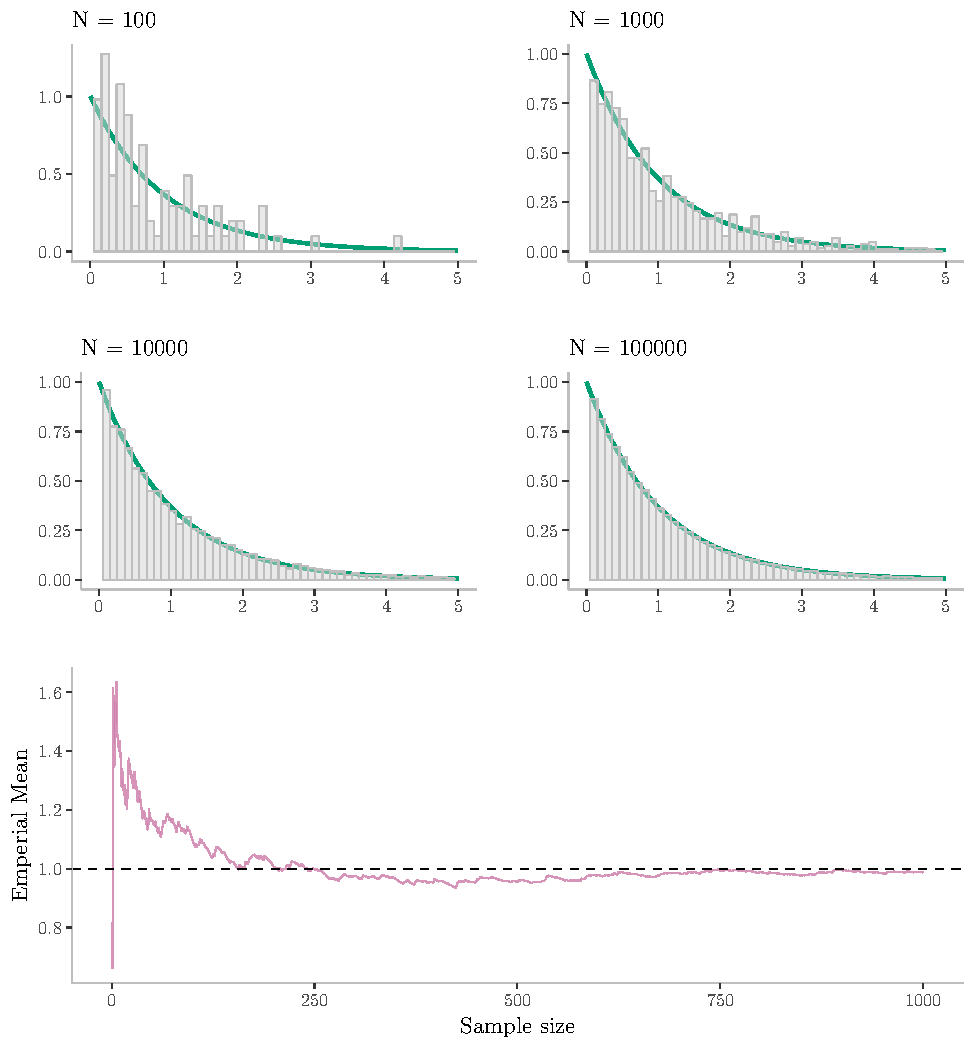
\includegraphics{thesis_files/figure-latex/unnamed-chunk-7-1.pdf}
\caption{\label{fig:unnamed-chunk-7}Above: Emperical distributions generated
by samples \(X_i \sim \text{Exp}(1)\) for \(i = 1, \ldots, N\) for \(N\)
of varying order of magnitude with exact \(\text{Exp}(1)\) distribution
plotted in green. Below: Convergence of the empirical mean, in pink, to
the true mean plotted as dashed grey line. \label{fig:monte}}
\end{figure}

\section{Markov chain Monte Carlo}\label{markov-chain-monte-carlo}

It is typically not possible to generate independent samples from the
relevant distribution directly. This is especially true for complex
models and in high dimensions, as with Markov melding.

Markov chain Monte Carlo (MCMC) is a flexible and broad class of
algorithms for sampling from probability distributions unable to be
sampled from directly. In MCMC, rather than drawing independent samples,
the sample at iteration \(i\) depends on that of the previous iteration
\(i-1\); the result being a a Markov chain of samples. By careful
specification, the stationary distribution of this Markov chain can be
set to correspond to the distribution \(\pi\). As a result, if the
Markov chain is run until it reaches convergence then it can
more-or-less be used in place of direct samples from \(\pi\). There are
many diagnostic tools which can be used to check if the chain appears to
have converged, the simplest being heuristic examinination of
trace-plots which show the positions of the chain over time. However,
convergence is not something which is possible to prove so disgression
must be taken.

Due to dependence on the previous value, samples from a Markov chain are
typically positively correlated, thereby reducing the amount of
information each sample contains about \(\pi\). This autocorrelation
should be taken into account when calculating the standard error of
Monte carlo estimates, see for example Gelman, Rubin, and others
(\protect\hyperlink{ref-gelman1992inference}{1992}). One popular metric
of this sort is the effective sample size (ESS) (Robert and Casella
\protect\hyperlink{ref-robert2013monte}{2013}) which can be interpreted
as the number of independent samples the correlated samples would be
equivalent to.

\subsection{Metropolis-Hastings}\label{metropolis-hastings}

\begin{center}
\begin{tcolorbox}[title= Algorithm~\ref*{alg:mh}: Metropolis-Hastings sampler, colback=white, width=0.95\linewidth, sharp corners]
\begin{algorithm}[H]
Target density $\pi$, initialise $x^{(0)}$\;
\For{$i = 1, 2, \ldots, N$}{
  Set current value $x = x^{(i-1)}$\;
  Draw candidate value $x^\star \sim q(\cdot \, | \, x)$\;
  Draw $u \sim \mathcal{U}(0, 1)$\;
  Let $\alpha = \min (1, r)$, where $r = \frac{\pi(x^\star) / q(x^\star \, | \, x)}{\pi(x) / q(x  \, | \, x^\star)}$\;
  \uIf{$\alpha$ > $u$}{
  $x^{(i)}=x^\star$\;
  }
  \uElse{
  $x^{(i)}=x$\;
  }
}
\caption{}
\label{alg:mh}
\end{algorithm}
\end{tcolorbox}
\end{center}

The Metropolis-Hastings (MH) algorithm dates back to foundational work
of Metropolis et al.
(\protect\hyperlink{ref-metropolis1953equation}{1953}) and Hastings
(\protect\hyperlink{ref-hastings1970monte}{1970}). At each iteration
\(i\), the next step \(x^\star\) is suggested according to a
user-specified proposal distribution \(q(\cdot \, | \, x)\) conditional
on the current location \(x = x^{(i-1)}\). Candidate values \(x^\star\)
are accepted with probability \(\alpha\), else the Markov chain remains
at the current location \(x\). The value of the acceptance probability
\(\alpha\) is calculated by

\begin{align}
\alpha &= \mathbb{P}[x^\star \text{ accepted}] 
= \min (1, r) \nonumber \\
&= \min \left(1, \frac{R(x^\star, x)}{R(x, x^\star)}\right)
= \min \left(1, \frac{\pi(x^\star) / q(x^\star \, | \, x)}{\pi(x) / q(x  \, | \, x^\star)}\right), \label{eq:acceptr}
\end{align}

where \(r\) is the ratio of target-to-proposal density ratios \(R\) at
the candidate \(x^\star\) and current \(x\) values.

In Bayesian statistics typically the target distribution \(\pi\) is such
that

\begin{equation}
\pi(x) = \frac{\gamma(x)}{Z}, \label{eq:normconst}
\end{equation}

where the normalising constant \(Z = \int \gamma(x) dx\) is
computationally intractable. To be specific, \(\pi\) is the product of
the likelihood and prior and \(Z\) is the marginal likelihood.
Therefore, it is crucial that Equation \eqref{eq:acceptr} only requires
the point-wise evaluation of \(\gamma\) and not \(\pi\) since
\(\pi(x)/\pi(z) = \gamma(x)/\gamma(z)\).

The efficiency of MH depends greatly on the user's choice of proposal
distribution \(q(\cdot \, | \, x)\). A common option is to consider
proposal distributions which are symmetric about the current value
\(x\), thereby simplifying the acceptance probability
\(\alpha = \min \left\{1, \pi(x^\star)/\pi(x)\right\}\) since
\(q(x \, | \, x^\star) = q(x^\star \, | \, x)\). This algorithm is
called random walk Metropolis (RWM). Roberts, Gelman, and Gilks
(\protect\hyperlink{ref-roberts1997weak}{1997}) show that, under certain
conditions, the acceptance rate for RWM which minimises autocorrelation
is 0.44 for one-dimensional proposals tending asymptotically to 0.234 as
the dimension increases.

By setting
\(\pi(x) = p_{\text{meld}}(\phi, \psi_1, \ldots, \psi_M \, | \, y_1, \ldots, y_M)\)
the general MH algorithm can be applied to target the Markov melded
posterior. The proposal distribution is then of the form
\(q(\phi^\star, \psi_1^\star, \ldots, \psi_M^\star \, | \, \phi, \psi_1, \ldots, \psi_M)\),
where \((\phi^\star, \psi_1^\star, \ldots, \psi_M^\star)\) are the
candidate values and \((\phi, \psi_1, \ldots, \psi_M)\) are the current
values of the chain.

The acceptance probability \(\alpha = \min (1, r)\) for moves
\((\phi, \psi_1, \ldots, \psi_M) \to (\phi^\star, \psi_1^\star, \ldots, \psi_M^\star)\)
can be calculated via

\begin{equation}
r=\frac{R(\phi^\star, \psi_1^\star, \ldots, \psi_M^\star, \phi, \psi_1, \ldots, \psi_M)}
       {R(\phi, \psi_1, \ldots, \psi_M, \phi^\star, \psi_1^\star, \ldots, \psi_M^\star)}, \label{eq:acceptprob}
\end{equation}

where
\(R(\phi^\star, \psi_1^\star, \ldots, \psi_M^\star, \phi, \psi_1, \ldots, \psi_M)\)
is the target-to-proposal density ratio

\begin{equation}
R(\phi^\star, \psi_1^\star, \ldots, \psi_{M}^\star, \phi, \psi_1, \ldots, \psi_{M}) 
= \frac{p_{\mathrm{pool}}(\phi^\star) \prod_{m=1}^{M} \frac{p_m(\phi^\star, \psi_m^\star, y_m)}{p_m(\phi^\star)}}{q(\phi^\star, \psi_1^\star, \ldots, \psi_{M}^\star \, | \, \phi, \psi_1, \ldots, \psi_{M})}
\end{equation}

For Markov melding, due to the possible quantity of parameters
\((\phi, \psi_1, \ldots, \psi_{M})\), it is likely difficult to find a
suitable choice of proposal distribution
\(q(\phi^\star, \psi_1^\star, \ldots, \psi_{M}^\star \, | \, \phi, \psi_1, \ldots, \psi_{M})\)
such that moves are accepted with reasonable probability.

\subsection{Metropolis-within-Gibbs}\label{metropolis-within-gibbs}

The general MH algorithm ignores the modular structure of the submodels.
As a result both of this structure and the difficulty of full parameter
moves, it may be more appealing to update submodel components
separately.

Gibbs sampling (S. Geman and Geman
\protect\hyperlink{ref-geman1987stochastic}{1987}) is an MCMC algorithm
which updates componentwise. In fact, Gibbs sampling is a special case
of MH where the acceptance rate can be calculated to be identically one.
Returning to the more general notation, suppose that \(x\) can be
written as a \(p\)-dimensional vector such that
\(x = (x_1, \ldots, x_p)\). In Gibbs sampling at each iteration \(i\)
only one of the components \(x_j\) where \(j \in 1, \ldots p\) is
updated. In particular, \(x_j\) is sampled from its full conditional
distribution, defined as

\begin{equation}
\pi_{X_j \, | \, X_{-j}} (x_j | x_{-j}) = \frac{\pi(x)}{\int \pi(x) dx_j}, \label{eq:fullconditional}
\end{equation}

where the notation \(x_{-j}\) refers to the subvector of \(x\) excluding
the \(j\)th element. There are multiple ways of choosing the component
\(j\) to update at each iteration: it can be chosen uniformly using
random-scan Gibbs sampling, or iterated over deterministically using
systematic-scan Gibbs sampling. Having selected a component to update
\(x_j\), informally speaking Gibbs sampling moves perpendicular to the
directions spanned by each of the other components \(x_{-j}\). If
components \(x_j\) and \(x_k\) are say positively correlated then
increases in \(x_j\) are typically accompanied by increases in
\(x_k, k \neq j\). In this situation, Gibbs sampling may not be
efficient as it struggles to find the relevant region using
perpendicular moves.

From a computational point of view, requiring that the full conditionals
of \(\pi\) are available and can be sampled from is often restrictive.
For Markov melding, the full conditionals of \(p_\text{meld}\) may not
be available and as a result generic Gibbs sampling is not generally
applicable. Instead, Goudie et al.
(\protect\hyperlink{ref-goudie2019joining}{2019}) propose the use of the
Metropolis-within-Gibbs (Muller
\protect\hyperlink{ref-muller1991generic}{1991}) (MWG) algorithm.

\begin{center}
\begin{tcolorbox}[title= Algorithm~\ref*{alg:mwg}: (Random-scan) Metropolis-within-Gibbs sampler, colback=white, width=0.95\linewidth, sharp corners]
\begin{algorithm}[H]
Target density $\pi$, initialise $x^{(0)} :=(x_{1}^{(0)}, \ldots, x_{p}^{(0)})$\;
\For{$i = 1, 2, \ldots, N$}{
  Set current value $x = x^{(i-1)}$\;
  Draw $j \sim \mathcal{U}\{1, \ldots, p\}$\;
  Draw $x^\star_{j} \sim q_j(\cdot \, | \, x)$\;
  Set $x^\star = (x_1, \ldots, x_j^\star, \ldots,  x_p)$\;
  Draw $u \sim \mathcal{U}(0, 1)$\;
  Let $\alpha = \min (1, r)$, where $r = \frac{\gamma(x^\star) / q(x^\star \, | \, x)}{\gamma(x) / q(x  \, | \, x^\star) \cdot }$\;
  \uIf{$\alpha$ > $u$}{
  $x^{(i)}=x^\star$\;
  }
  \uElse{
  $x^{(i)}=x$\;
  }
}
\caption{}
\label{alg:mwg}
\end{algorithm}
\end{tcolorbox}
\end{center}

MWG unifies MH and Gibbs sampling by utilising componentwise MH
proposals rather than sampling from the full conditionals exactly. As
such, MWG does not require access to the full conditionals and as a
result is more generally applicable. Of course, if for some index \(j\)
the full conditional is available then it is a valid MH update and can
be used.

As with MH, the user must specify the proposal distributions, in this
case \(q_j(\cdot \, | \, x_j^{(i-1)})\) for each of the \(p\)
components. For random walk type proposals the resulting algorithm known
as random walk Metropolis-within-Gibbs (RWM-within-Gibbs). This
algorithm is studied in the context of optimal scaling by Neal and
Roberts (\protect\hyperlink{ref-neal2006optimal}{2006}) who show that,
as with RWM, the optimal acceptance rate is 0.44 for one-dimensional
proposals again tending to 0.234 for higher dimension as with Roberts,
Gelman, and Gilks (\protect\hyperlink{ref-roberts1997weak}{1997}).

Now, to target Equation \eqref{eq:meldpost} using MWG, define the
components of \((\phi, \psi_1, \ldots, \psi_M)\) be the link parameter
\(\phi\) and each of the model specific parameters \(\psi_m\),
\(m = 1, \ldots, M\) respectively as would be expected. Suppose the
initial values \((\phi^{(0)}, \psi_1^{(0)}, \ldots, \psi_M^{(0)})\) are
given.

\textbf{Model specific parameter updates} In Markov melding, it is
assumed \eqref{eq:cindep} that the \(\psi_m\) are conditionally
independent given \(\phi\). Supposing this assumption is reasonable, it
would therefore be expected that Gibbs and MWG sampling would be
relatively efficient for model specific parameters. For each of
\(\psi_m\) for \(m = 1, \ldots, M\) define a proposal distribution
\(q_m(\cdot \, | \, \psi_m)\). The target-to-proposal density ratio is
then

\begin{align}
&\phantom{=} R(\phi, \psi_1, \ldots, \psi_m^\star, \ldots, \psi_M, \phi, \psi_1, \ldots, \psi_m, \ldots, \psi_M) \nonumber \\
&= p_{\mathrm{pool}}(\phi) \prod_{j=1}^M \frac{p_j(\phi, \psi_j, y_j)}{p_j(\phi)} \frac{1}{q_m(\psi_m^\star \, | \, \psi_m)} \nonumber \\
&= p_{\mathrm{pool}}(\phi) \prod_{j\neq m} \frac{p_j(\phi, \psi_j, y_j)}{p_j(\phi)} \cdot \frac{p_m(\phi, \psi_m^\star, y_m)}{p_m(\phi)} \frac{1}{q_m(\psi_m^\star \, | \, \psi_m)}.
\end{align}

In calculating \(r\) via \eqref{eq:acceptprob} factors not dependent on
submodel \(m\), as well as the pooled prior, cancel leaving

\begin{equation}
r = \frac{p_m(\phi, \psi_m^\star, y_m) \cdot \frac{1}{q_m(\psi_m^\star \, | \, \psi_m)}}{p_m(\phi, \psi_m, y_m) \cdot \frac{1}{q_m(\psi_m \, | \, \psi_m^\star)}}. \label{eq:latentupdate}
\end{equation}

Equation \eqref{eq:latentupdate} precisely corresponds to updating
\(\psi_m\) conditional on the link parameter \(\phi\) for inference
performed on the \(m\)\textsuperscript{th} alone. With each submodel
having been specified as it is, it's reasonable to expect that inference
for each submodel individually is tractable via MH. As such, it is
possible to calculate the ratio in Equation \eqref{eq:latentupdate} for
each \(m = 1, \ldots, M\).

\textbf{Link parameter updates} In contrast to the above, one would
expect the link parameter \(\phi\) to have covariance structure with
each of the model specific parameters: potentially making link parameter
updates relatively inefficient. For the link parameter \(\phi\) define a
proposal distribution \(q(\cdot \, | \, \phi)\). The target-to-proposal
density ratio is

\begin{equation}
R(\phi, \psi_1, \ldots, \psi_M, \phi^\star, \psi_1, \ldots, \psi_M) = p_{\mathrm{pool}}(\phi^\star) \prod_{m=1}^M \frac{p_m(\phi^\star, \psi_m, y_m)}{p_m(\phi^\star)} \cdot \frac{1}{q(\phi^\star \, | \, \phi)}. \label{eq:linkttp}
\end{equation}

If Product of Experts pooling is used then the marginal distributions of
the link parameter cancel, leaving

\begin{align}
R(\phi, \psi_1, \ldots, \psi_M, \phi^\star, \psi_1, \ldots, \psi_M) 
&\propto \prod_{m=1}^M p_m(\phi^\star) \prod_{m=1}^M \frac{p_m(\phi^\star, \psi_m, y_m)}{p_m(\phi^\star)} \cdot \frac{1}{q(\phi^\star \, | \, \phi)} \nonumber \\
&= \prod_{m=1}^M p_m(\phi^\star, \psi_m, y_m) \cdot \frac{1}{q(\phi^\star \, | \, \phi)}.
\end{align}

However, in general, in order to calculate Equation \eqref{eq:linkttp}
the prior marginal distributions \(p_m(\phi)\) and the closely related
\(p_{\mathrm{pool}}\) must be evaluated. If \(p_m(\phi)\) is not
tractable, Goudie et al.
(\protect\hyperlink{ref-goudie2019joining}{2019}) suggest using an
approximation \(\hat p_m(\phi)\) found using kernel density estimation
with samples drawn from the prior marginal given by Equation
\eqref{eq:priormarginal}. Samples can be drawn by forward Monte Carlo:
simulating the statistical relationships (which typically are standard
distributions) top-down in the DAG representation of the submodel until
the node corresponding to \(\phi\) is reached.

In the following example, we demonstrate the use of MCMC for Markov
melding two different types of meta-analysis.

\emph{Example 3.2: Metropolis-within-Gibbs for Markov melding}

\begin{figure}
\centering
\begin{tikzpicture}[
      > = stealth, % arrow head style
      shorten > = 1pt, % don't touch arrow head to node
      auto,
      node distance = 3cm, % distance between nodes
      semithick % line style
    ]

    \node[constant] (1) at (0,0){$\kappa_0$};
    \node[constant] (2) at (2,0) {$\upsilon_0$};
    \node[state] (3) at (1,-2) {$\kappa$};
    
    \node[constant] (4) at (4,0){$a$};
    \node[constant] (5) at (6,0) {$b$};
    \node[state] (6) at (5,-2) {$\upsilon$};
    
    \node[state] (7) at (3,-4) {$\delta_i$};
    
    \node[constant] (8) at (7,-2){$\mu_0$};
    \node[constant] (9) at (9,-2) {$\tau_0$};
    \node[state] (10) at (8,-4) {$\mu_i$};
    
    \node[state] (11) at (4.5,-6) {$p_i^C$};
    \node[state] (12) at (6.5,-6) {$p_i^T$};
            
    \node[state] (13) at (4.5,-8) {$r_i^C$};            
    \node[state] (14) at (6.5,-8) {$r_i^T$};
    
    \node[constant] (15) at (0.5,-6) {$N_1$};
    
    \node[above right] at (1.5, -9) {$i = 1, \ldots, n_1$}; 

    \path (1) edge  (3);
    \path (2) edge  (3);
    
    \path (4) edge  (6);
    \path (5) edge  (6);
    
    \path (3) edge  (7);
    \path (6) edge  (7);
    
    \path (8) edge  (10);
    \path (9) edge  (10);
    
    \path (7) edge  (11);
    \path (7) edge  (12);
    \path (10) edge  (11);
    \path (10) edge  (12);
    
    \path (11) edge  (13);
    \path (12) edge  (14);
    \path (15) edge  (13);
    \path (15) edge  (14);
    
    \draw (1.5,-3) -- (9.5,-3) -- (9.5,-9) -- (1.5,-9) -- cycle;
\end{tikzpicture}
\caption{DAG representing Submodel 1}
\label{fig:ex2dag1}
\end{figure}

\textbf{Submodel 1} Standard meta-analysis usually assumes that either
effects are common across studies (fixed-effects) or drawn from a
probability distribution (random-effects). T. Smith, Spiegelhalter, and
Thomas (\protect\hyperlink{ref-smith1995bayesian}{1995}) present a fully
Bayesian approach to random-effects meta-analysis. They use this model
to study the effectiveness of a treatment (selective decontamination of
the digestive tract) which aims to prevent patients acquiring infections
whilst in intensive care units (ICUs). We present an adapted version of
the model as follows.

Consider \(n_1 = 5\) trials \(i = 1, \ldots, n_1\) each with both a
control (\(C\)) and treatment (\(T\)) group of size \(N_1 = 10\). In
trial \(i\), individuals within group \(j \in \{C, T\}\) are assumed to
have independent probability \(p_i^j\) of developing an infection. The
numbers of infections in the control and treatment groups for trial
\(i\) are \(r_i^C\) and \(r_i^T\) respectively. Assume that \(\mu_i\) is
the average infection rate for the \(i\)\textsuperscript{th} trial and
\(\delta_i\) is the true treatment effect, both on the log-odds scale.
Following T. Smith, Spiegelhalter, and Thomas
(\protect\hyperlink{ref-smith1995bayesian}{1995}), we place an
uninformative Gaussian prior on each \(\mu_i\), with fixed prior mean
\(\mu_0 = 0\) and precision \(\tau_0 = 0.25\) hyperparameters. The prior
on each \(\delta_i\) is also Gaussian mean \(\kappa\) and precision
\(\tau\). Uninformative hyperpriors \eqref{eq:hyperprior1} and
\eqref{eq:hyperprior2} are placed on both \(\kappa\) and \(\tau\) with
\(\kappa_0 = 0\), \(\tau = 0.1\), \(a = 3\), \(b = 1\). Clinical trials
aim to assess treatment effectiveness and therefore the mean (log-odds
scale) treatment effect \(\kappa\) is the parameter of interest. The
full model \(p_1(\kappa, \upsilon, \delta, \mu, p^C, p^T, r^C, r^T)\) is
then

\begin{align}
\kappa &\sim \mathcal{N}(\kappa_0, \upsilon_0^{-1}), \label{eq:hyperprior1} \\
\upsilon &\sim \text{Gamma}(a, b), \label{eq:hyperprior2} \\
\delta_i &\sim \mathcal{N}(\kappa, \upsilon^{-1}), \\
\mu_i &\sim \mathcal{N}(\mu_0, \tau_0^{-1}), \\
p_i^C &= \frac{e^{\mu_i - \delta_i/2}}{1 + e^{\mu_i - \delta_i/2}}, \; p_i^T = \frac{e^{\mu_i + \delta_i/2}}{1 + e^{\mu_i + \delta_i/2}}, \\
r_i^C &\sim \text{Bin}(N_1, p_i^C), \; r_i^T \sim \text{Bin}(N_1, p_i^T), \quad i = 1, \ldots, n_1,
\end{align}

where the vectors \(\delta, \mu, p^C, p^T, r^C, r^T\) are each of length
\(n_1\), e.g. \(\delta = (\delta_1, \ldots, \delta_{n_1})\). Observed
data for Submodel 1 is \(Y_1 = (r^C, r^T)\). For this example, we
forward simulate the observed data \(Y_1 = y_1\) (with \(N_1 = 10\) and
\(n_1 = 5\)) from
\(\delta_i \sim \mathcal{N}(-0.25, 4^{-1}), \; \mu_i \sim \mathcal{N}(-1, 2^{-1})\),
resulting in
\(r^C = \{8, 8, 11, 6, 5 \}, \; r^T = \{2, 2, 5, 11, 4 \}\).

The probabilities \(p = (p_i^C, p_i^T)\) are an (invertible)
deterministic transformation of \((\mu_i, \delta_i)\). Therefore, each
probability has an induced distribution via Equation
\eqref{eq:transform}. Had a prior been specified on \(p\) then the
situation would have been identical to that of Poole and Raftery
(\protect\hyperlink{ref-poole2000inference}{2000}) where there exist
multiple priors on parameters in a deterministic simulation model. To
resolve issues of this sort Goudie et al.
(\protect\hyperlink{ref-goudie2019joining}{2019}) propose using Bayesian
melding (introduced in Section \ref{sec:bayesianmelding}) however in
this instance we choose not to place a prior on \(p\); implicitly
accepting the distribution induced by \(\mu_i\) and \(\delta_i\). In
particular, for \(p_i^C\) (a similar statement is true for \(p_i^T\)) we
have the inverse transformation

\begin{equation}
\mu_i - \delta_i/2 = \text{logit}(p_i^C) = \log \frac{p_i^C}{1 - p_i^C},
\end{equation}

with corresponding Jacobian

\begin{equation}
\left|\frac{\delta (\mu_i - \delta_i/2)}{\delta p_i}\right| = \frac{1}{p_i^C(1-p_i^C)}.
\end{equation}

As linear transformations of Gaussian distributions,
\(\mu_i \pm \delta_i/2\) are Gaussian with mean and variance given by

\begin{align}
\mathbb{E}[\mu_i - \delta_i/2 | \mu_0, \tau_0, \kappa, \upsilon] &= \mu_0 - \kappa/2, \\
\mathbb{E}[\mu_i + \delta_i/2 | \mu_0, \tau_0, \kappa, \upsilon] &= \mu_0 + \kappa/2, \\
\mathbb{V}[\mu_i \pm \delta_i/2 | \mu_0, \tau_0, \kappa, \upsilon] &= \tau_0^{-1} + \upsilon^{-1}/4.
\end{align}

Therefore, defining \((\tau_0^{-1} + \upsilon^{-1}/4)^{-1} = \omega\),
the distributions of \(p_i^C\) and \(p_i^T\) are given by

\begin{align}
p(p_i^C \, | \, \mu_0, \tau_0, \kappa, \upsilon) &= \frac{\omega}{\sqrt{2\pi}} \exp\left(-\frac{\omega}{2}\left(\log \frac{p_i^C}{1 - p_i^C} - (\mu_0 - \kappa/2)\right)^2\right) \frac{1}{p_i^C(1-p_i^C)}, \label{eq:piC} \\
p(p_i^T \, | \, \mu_0, \tau_0, \kappa, \upsilon) &= \frac{\omega}{\sqrt{2\pi}} \exp\left(-\frac{\omega}{2}\left(\log \frac{p_i^T}{1 - p_i^T} - (\mu_0 + \kappa/2)\right)^2\right) \frac{1}{p_i^T(1-p_i^T)}. \label{eq:piT}
\end{align}

Having calculated distributions \eqref{eq:piC} and \eqref{eq:piT}
dependence on \((\mu, \delta)\) can be omitted. Given \((r^C, r^T)\)
(and additionally omitting dependence on fixed hyperparameters) the
posterior distribution is then

\begin{align}
&\phantom{\propto} p_1(\kappa, \upsilon, p^C, p^T \, | \, r^C, r^T) \nonumber \\
&\propto \prod_{i=1}^{n_1} {N_1\choose r_i^C} {p_i^C}^{r_i^C} (1 - p_i^C)^{N_1 - r_i^C} \frac{\omega}{\sqrt{2\pi}} \exp\left(-\frac{\omega}{2}\left(\log \frac{p_i^C}{1 - p_i^C} - (\mu_0 - \kappa/2)\right)^2\right) \frac{1}{p_i^C(1-p_i^C)} \nonumber \\
&\phantom{\propto} \cdot \prod_{i=1}^{n_1} {N_1\choose r_i^T} {p_i^T}^{r_i^T} (1 - p_i^T)^{N_1 - r_i^T}
\frac{\omega}{\sqrt{2\pi}} \exp\left(-\frac{\omega}{2}\left(\log \frac{p_i^T}{1 - p_i^T} - (\mu_0 + \kappa/2)\right)^2\right) \frac{1}{p_i^T(1-p_i^T)} \nonumber \\
&\phantom{\propto} \cdot \frac{\tau_0}{\sqrt{2\pi}} \exp\left(-\frac{\tau_0}{2}(\mu - \mu_0)^2\right) \cdot \frac{b^a}{\Gamma(a)} \tau^{a-1} \exp(-b \tau) \nonumber \\
% New line
&\propto \prod_{i=1}^{n_1} \{ {p_i^C}^{r_i^C - 1} (1 - p_i^C)^{N_1 - r_i^C - 1} \} \, \omega^{n_1} \exp\left(-\frac{\omega}{2} \sum_{i=1}^{n_1} \left(\log \frac{p_i^C}{1 - p_i^C} - (\mu_0 - \kappa/2)\right)^2\right) \nonumber \\
&\phantom{\propto} \cdot \prod_{i=1}^{n_1} \{ {p_i^T}^{r_i^T - 1} (1 - p_i^T)^{N_1 - r_i^T - 1} \} \, \omega^{n_1} \exp\left(-\frac{\omega}{2} \sum_{i=1}^{n_1} \left(\log \frac{p_i^T}{1 - p_i^T} - (\mu_0 + \kappa/2)\right)^2\right) \nonumber \\
&\phantom{\propto} \cdot \exp\left(-\frac{\upsilon_0}{2}(\kappa - \kappa_0)^2\right) \upsilon^{a-1} \exp(-b \upsilon) \label{eq:ex2post}
\end{align}

Often it is more computationally convenient to work in terms of
logarithms as this allows products to be replaced with sums. The
log-posterior is

\begin{align}
&\phantom{\propto} \log p(\kappa, \upsilon, p^C, p^T \, | \, r^C, r^T) \nonumber \\
&\propto \sum_{i = 1}^{n_1} \{ (r_i^C - 1) \log p_i^C + (N_1 - r_i^C - 1) \log (1 - p_i^C) \nonumber \\
&\phantom{\propto} + (r_i^T - 1) \log p_i^T + (N_1 - r_i^T - 1) \log (1 - p_i^T) \nonumber \\
&\phantom{\propto} - \frac{\omega}{2} \left(\log \frac{p_i^C}{1 - p_i^C} - (\mu_0 - \kappa/2)\right)^2 - \frac{\omega}{2} \left(\log \frac{p_i^T}{1 - p_i^T} - (\mu_0 + \kappa/2)\right)^2 \} \nonumber \\
&\phantom{\propto} + 2n_1 \omega - \frac{\upsilon_0}{2}(\kappa - \kappa_0)^2 + (a - 1)\log \upsilon - b \upsilon := \ell_1
\end{align}

To target the posterior \eqref{eq:ex2post} we use RWM-within-Gibbs. The
initialisation values are chosen to be \(0.5\) for each of the
probabilities and otherwise chosen according to the prior means
\((\kappa^{(0)}, \upsilon^{(0)}) = (\kappa_0, a/b) = (0, 1/3)\). The
proposal distribution for each component is Gaussian with indivual
componentwise standard deviation parameters tuned to achieve close to
the optimal one-dimensional acceptance rate 0.44 (Roberts, Gelman, and
Gilks (\protect\hyperlink{ref-roberts1997weak}{1997}) note that there is
``little value'' in finely tuning algorithms to exact values).

\begin{table}[!h]

\caption{\label{tab:unnamed-chunk-9}Scaling and resultant acceptance rates for each component.}
\centering
\resizebox{\linewidth}{!}{
\begin{tabular}{lrrrrrrrrrrrr}
\toprule
  & $\kappa$ & $\upsilon$ & $p_1^C$ & $p_2^C$ & $p_3^C$ & $p_4^C$ & $p_5^C$ & $p_1^T$ & $p_2^T$ & $p_3^T$ & $p_4^T$ & $p_5^T$\\
\midrule
$\sigma$ & 3.000 & 3.500 & 0.300 & 0.250 & 0.300 & 0.250 & 0.200 & 0.150 & 0.150 & 0.250 & 0.300 & 0.200\\
Acceptance & 0.427 & 0.452 & 0.384 & 0.407 & 0.398 & 0.381 & 0.411 & 0.438 & 0.437 & 0.406 & 0.397 & 0.447\\
\bottomrule
\end{tabular}}
\end{table}

To determine an appropriate number of Markov chain samples for the
problem at hand one method is to consider the ESS. To this end, Vats,
Flegal, and Jones (\protect\hyperlink{ref-vats2015multivariate}{2015})
calculate a lower bound on the number of effective samples required to
estimate a vector of length \(p\) with \(100(1 - \alpha)\%\) confidence
and a relative tolerance of \(\epsilon\). Additionally, they define a
multivariate ESS which takes into account cross-correlation across the
Markov chain components. Both these methods are implemented in the
\texttt{R} package \texttt{mcmcse} (J. M. Flegal et al.
\protect\hyperlink{ref-mcmcse}{2017}).

In order to estimate the mean, of length \(p = 12\), with \(97.5\%\)
confidence and a tolerance of \(\epsilon = 0.025\) the required number
of effective samples is approximately 40000. Based on a short trial
chain, the number of simulations required to achieve this ESS is 2800000
(although this may seem high, at every iteration only one component is
proposed and therefore the chain is highly auto-correlated). That being
said, the algorithm is not prohibitively computationally intensive, so
we choose to run 5000000 iterations.

\begin{table}[!h]

\caption{\label{tab:unnamed-chunk-10}Posterior mean (PM), true value and posterior standard deviation (PSD) for each component.}
\centering
\resizebox{\linewidth}{!}{
\begin{tabular}{lrrrrrrrrrrrr}
\toprule
  & $\kappa$ & $\upsilon$ & $p_1^C$ & $p_2^C$ & $p_3^C$ & $p_4^C$ & $p_5^C$ & $p_1^T$ & $p_2^T$ & $p_3^T$ & $p_4^T$ & $p_5^T$\\
\midrule
PM & -0.314 & 2.991 & 0.359 & 0.265 & 0.502 & 0.219 & 0.172 & 0.124 & 0.124 & 0.262 & 0.546 & 0.215\\
Truth & -0.250 & 4.000 & 0.214 & 0.360 & 0.464 & 0.296 & 0.236 & 0.134 & 0.324 & 0.308 & 0.421 & 0.221\\
PSD & 1.229 & 1.731 & 0.102 & 0.093 & 0.106 & 0.088 & 0.079 & 0.068 & 0.069 & 0.093 & 0.107 & 0.087\\
\bottomrule
\end{tabular}}
\end{table}

\begin{figure}
\centering
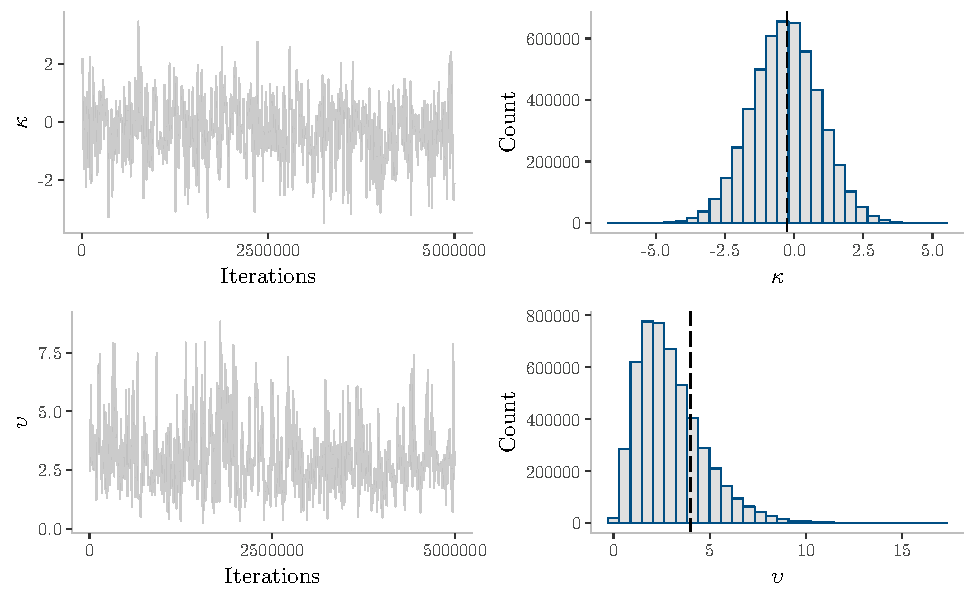
\includegraphics{thesis_files/figure-latex/unnamed-chunk-11-1.pdf}
\caption{\label{fig:unnamed-chunk-11}Submodel 1 posterior traceplots and
histograms for the parameters \(\kappa\) and \(\upsilon\), with truth
shown on the histogram as a dashed black line. Similar plots for the ten
other probability parameters are presented in Appendix \ref{app:A}. Note
that for this, and all subsequent, traceplots the chains have first been
thinned for graphical display reasons.}
\end{figure}

\newpage

\begin{figure}
\centering
\begin{tikzpicture}[
      > = stealth, % arrow head style
      shorten > = 1pt, % don't touch arrow head to node
      auto,
      node distance = 3cm, % distance between nodes
      semithick % line style
    ]

    \node[constant] (1) at (0,0){$\kappa_0$};
    \node[constant] (2) at (2,0) {$\upsilon_0$};
    \node[state] (3) at (1,-2) {$\kappa$};
    
    \node[constant] (4) at (4,0){$\lambda_0$};
    \node[constant] (5) at (6,0) {$\gamma_0$};
    \node[state] (6) at (5,-2) {$\lambda$};
    
    \node[state] (7) at (2,-4) {$q^C$};
    \node[state] (8) at (4,-4) {$q^T$};
    
    \node[state] (9) at (2,-6) {$s_i^C$};
    \node[state] (10) at (4,-6) {$s_i^T$};
    
    \node[constant] (11) at (0,-4) {$N_2$};
    
    \node[above right] at (1, -7.25) {$i = 1, \ldots, n_2$}; 

    \path (1) edge  (3);
    \path (2) edge  (3);
    
    \path (4) edge  (6);
    \path (5) edge  (6);
    
    \path (3) edge  (7);
    \path (6) edge  (7);
    \path (3) edge  (8);
    \path (6) edge  (8);
    
    \path (7) edge  (9);
    \path (8) edge  (10);
    \path (11) edge  (9);
    \path (11) edge  (10);
    
    
    \draw (1,-5) -- (5,-5) -- (5,-7.25) -- (1,-7.25) -- cycle;
\end{tikzpicture}
\caption{DAG representing Submodel 2}
\label{fig:ex2dag2}
\end{figure}

\textbf{Submodel 2} For the second submodel we consider a fixed-effects
meta-analysis. The full model
\(p_2(\kappa, \lambda, q^C, q^T, r^C, r^T)\) is given by

\begin{align}
\kappa &\sim \mathcal{N}(\kappa_0, \upsilon_0^{-1}),  \\
\lambda &\sim \mathcal{N}(\lambda_0, \gamma_0^{-1}), \\
q^C &= \frac{e^{\lambda - \kappa/2}}{1 + e^{\lambda - \kappa/2}}, \; q^T = \frac{e^{\lambda + \kappa/2}}{1 + e^{\lambda + \kappa/2}}, \\
s_i^C &\sim \text{Bin}(N_2, q^C), \; s_i^T \sim \text{Bin}(N_2, q^T), \quad i = 1, \ldots, n_2.
\end{align}

To facilitate Markov melding, inference about the underlying parameters
\(\kappa\) and \(\lambda\) is conducted rather than the probabilies
\(q^C\) and \(q^T\) - which typically would seem to be the more natural
option. Indeed for a fixed effects meta-analysis more generally it would
likely be preferable to directly place priors on the probabilies (for
example a Beta prior would be conjugate to the Binomial likelihood).
Setting this fact aside, the posterior distribution given \((s^C, s^T)\)
is

\begin{align}
&\phantom{\propto} p_2(\kappa, \lambda \, | \, s^C, s^T) \nonumber \\
&\propto \prod_{i = 1}^{n_2} {N_2\choose s_i^C} \left(\frac{e^{\lambda - \kappa/2}}{1 + e^{\lambda - \kappa/2}}\right)^{s_i^C} \left(\frac{1}{1 + e^{\lambda - \kappa/2}}\right)^{N_2 - s_i^C} \left(\frac{1}{1 + e^{\lambda - \kappa/2}}\right)^2 \nonumber \\
&\phantom{\propto} \cdot \prod_{i = 1}^{n_2} {N_2\choose s_i^T} \left(\frac{e^{\lambda + \kappa/2}}{1 + e^{\lambda + \kappa/2}}\right)^{s_i^T} \left(\frac{1}{1 + e^{\lambda + \kappa/2}}\right)^{N_2 - s_i^T} \left(\frac{1}{1 + e^{\lambda + \kappa/2}}\right)^2 \nonumber \\
&\phantom{\propto} \cdot \frac{\upsilon_0}{\sqrt{2\pi}} \exp\left(-\frac{\upsilon_0}{2}(\kappa - \kappa_0)^2\right) \cdot \frac{\gamma_0}{\sqrt{2\pi}} \exp\left(-\frac{\gamma_0}{2}(\lambda - \lambda_0)^2\right) \nonumber \\
% End line
&\propto \left(\frac{e^{\lambda - \kappa/2}}{1 + e^{\lambda - \kappa/2}}\right)^{\sum_{i = 1}^{n_2} s_i^C} \left(\frac{1}{1 + e^{\lambda - \kappa/2}}\right)^{2 + n_2N_2 - \sum_{i = 1}^{n_2} s_i^C} \nonumber \\
&\phantom{\propto}  \cdot \left(\frac{e^{\lambda + \kappa/2}}{1 + e^{\lambda + \kappa/2}}\right)^{\sum_{i = 1}^{n_2} s_i^T} \left(\frac{1}{1 + e^{\lambda + \kappa/2}}\right)^{2 + n_2N_2 - \sum_{i = 1}^{n_2} s_i^T} \nonumber \\
&\phantom{\propto} \cdot  \exp\left(-\frac{\upsilon_0}{2}(\kappa - \kappa_0)^2\right) \cdot \exp\left(-\frac{\gamma_0}{2}(\lambda - \lambda_0)^2\right),
\end{align}

again using a transformation of variables (with Jacobians
\((1 + e^{\lambda - \kappa/2})^{-2}\)). The log posterior is

\begin{align}
&\phantom{\propto} = \log p(\kappa, \lambda \, | \, s^C, s^T) \nonumber \\
&\propto \sum_{i = 1}^{n_2} s_i^C \log \left(\frac{e^{\lambda - \kappa/2}}{1 + e^{\lambda - \kappa/2}}\right) + (2 + n_2N_2 - \sum_{i = 1}^{n_2} s_i^C) \log \left(\frac{1}{1 + e^{\lambda - \kappa/2}}\right) \nonumber \\
&\phantom{\propto} + \sum_{i = 1}^{n_2} s_i^T \log \left(\frac{e^{\lambda + \kappa/2}}{1 + e^{\lambda + \kappa/2}}\right) + (2 + n_2N_2 - \sum_{i = 1}^{n_2} s_i^T) \log \left(\frac{1}{1 + e^{\lambda + \kappa/2}}\right) \nonumber \\
&\phantom{\propto} - \frac{\upsilon_0}{2}(\kappa - \kappa_0)^2  - \frac{\gamma_0}{2}(\lambda - \lambda_0)^2 := \ell_2
\end{align}

\begin{table}[!h]

\caption{\label{tab:unnamed-chunk-13}Scaling and acceptance rate for $\kappa$ and $\lambda$.}
\centering
\begin{tabular}{lrr}
\toprule
  & $\kappa$ & $\lambda$\\
\midrule
$\sigma$ & 0.550 & 0.300\\
Acceptance & 0.472 & 0.452\\
\bottomrule
\end{tabular}
\end{table}

\begin{table}[!h]

\caption{\label{tab:unnamed-chunk-14}Posterior mean (PM), true value and posterior standard deviation (PSD) for $\kappa$ and $\lambda$.}
\centering
\begin{tabular}{lrr}
\toprule
  & $\kappa$ & $\lambda$\\
\midrule
PM & -0.303 & -1.021\\
Truth & -0.250 & -1.000\\
PSD & 0.253 & 0.131\\
\bottomrule
\end{tabular}
\end{table}

\begin{figure}
\centering
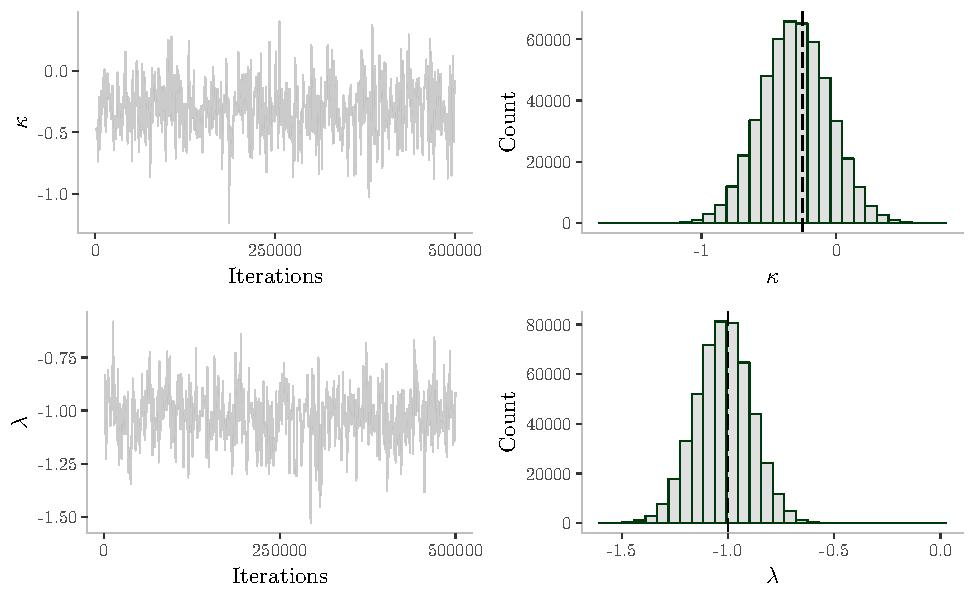
\includegraphics{thesis_files/figure-latex/unnamed-chunk-15-1.pdf}
\caption{\label{fig:unnamed-chunk-15}Submodel 2 posterior traceplots and
histograms for the parameters \(\kappa\) and \(\lambda\), with truth
shown on the histogram as a dashed black line.}
\end{figure}

\newpage

\textbf{Melded model}

\begin{align}
&\phantom{\propto} p_{\text{meld}}(\kappa, \upsilon, p^C, p^T, \lambda \, | \, r^C, r^T, s^C, s^T) \nonumber \\
&\propto p_{\text{pool}}(\kappa) \frac{p_1(\kappa, \upsilon, p^C, p^T \, | \, r^C, r^T)}{p_1(\kappa)} \frac{p_1(\kappa, \upsilon, p^C, p^T \, | \, r^C, r^T)}{p_2(\kappa)}
\end{align}

\begin{equation}
p_{\text{meld}}(\kappa, \upsilon, p^C, p^T, \lambda \, | \, r^C, r^T, s^C, s^T)
\propto p_1(\kappa, \upsilon, p^C, p^T \, | \, r^C, r^T) p_1(\kappa, \upsilon, p^C, p^T \, | \, r^C, r^T)
\end{equation}

\begin{align}
&\phantom{\propto} \log p_{\text{meld}}(\kappa, \upsilon, p^C, p^T, \lambda \, | \, r^C, r^T, s^C, s^T) \nonumber \\
&\propto \log p_1(\kappa, \upsilon, p^C, p^T \, | \, r^C, r^T) + \log p_2(\kappa, \upsilon, p^C, p^T \, | \, r^C, r^T) \nonumber \\
&\propto \ell_1 + \ell_2
\end{align}

\begin{verbatim}
## Warning in rbind(vscale, accept): number of columns of result is not a
## multiple of vector length (arg 1)
\end{verbatim}

\begin{table}[!h]

\caption{\label{tab:unnamed-chunk-17}Scaling and acceptance rate for $\kappa$ and $\lambda$.}
\centering
\begin{tabular}{lrrrrrrrrrrrrr}
\toprule
  & $\kappa$ & $\lambda$ & NA & NA & NA & NA & NA & NA & NA & NA & NA & NA & NA\\
\midrule
$\sigma$ & 0.550 & 0.300 & 0.550 & 0.300 & 0.550 & 0.300 & 0.550 & 0.300 & 0.550 & 0.300 & 0.550 & 0.300 & 0.550\\
Acceptance & 0.291 & 0.452 & 0.384 & 0.408 & 0.398 & 0.381 & 0.411 & 0.438 & 0.439 & 0.407 & 0.396 & 0.448 & 0.162\\
\bottomrule
\end{tabular}
\end{table}

\begin{figure}
\centering
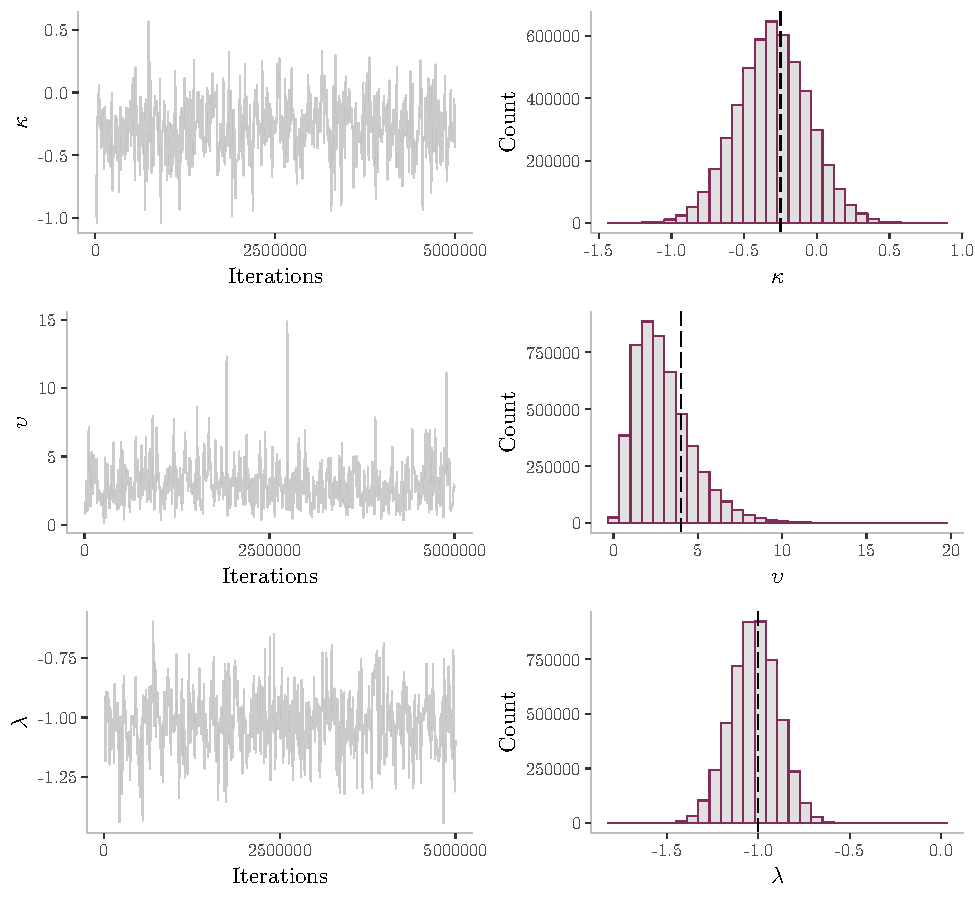
\includegraphics{thesis_files/figure-latex/unnamed-chunk-18-1.pdf}
\caption{\label{fig:unnamed-chunk-18}Melded model posterior traceplots and
histograms for the parameters \(\kappa\), \(\upsilon\) and \(\lambda\),
with truth shown on the histogram as a dashed black line.}
\end{figure}

\newpage

\section{Sequential Monte Carlo}\label{sequential-monte-carlo}

In some situations, where the submodels are complex, it may be
challenging to directly sample from the full Markov melded posterior
using Metropolis-within-Gibbs. Goudie et al.
(\protect\hyperlink{ref-goudie2019joining}{2019}) therefore propose a
sequential approach, in which information from the submodels is added
step-by-step. At a high-level, it is an example of Sequential Monte
Carlo (SMC) which we outline the connection to here.

Consider a probability density function \(\pi(x)\) as before defined on
the state space \(\mathcal{X}\). Following Lindsten et al.
(\protect\hyperlink{ref-lindsten2017divide}{2017}), if \(\mathcal{X}\)
is a product space it may be decomposed into a Cartesian product of
subspaces according to

\begin{equation}
\mathcal{X} := \mathcal{X}_T = \widetilde{\mathcal{X}}_1 \times \widetilde{\mathcal{X}}_2 \times \cdots \times \widetilde{\mathcal{X}}_T. \label{eq:seqdecomp}
\end{equation}

Elements \(x \in \mathcal{X}\) in the product space may be written as
\(x := x_T = (\widetilde{x}_1, \ldots, \widetilde{x}_T)\). Both the
elements of the subspaces and the subspaces themselves are denoted with
tildes, so that \(\widetilde{x}_t \in \widetilde{\mathcal{X}}_t,\) for
\(1 \leq t \leq T\). A sequence of auxiliary probability distributions
\(\pi_1, \ldots \pi_T\) can be defined on the spaces \(\mathcal{X}_t\)
of lower dimension \(1 \leq t \leq T\) than \(\mathcal{X}_T\).
\(\pi_t(x_t) := \pi_t(\widetilde{x}_1, \cdots, \widetilde{x}_t)\) for
\(t = 1, \ldots, T\). The final auxiliary distribution is chosen to
coincide with the target distribution, such that

\begin{equation}
\pi = \pi_T \label{eq:seqfinal}.
\end{equation}

Collections of auxiliary distributions with the two properties,
\eqref{eq:seqdecomp} and \eqref{eq:seqfinal}, are called a sequential
decomposition of the target distribution \(\pi\).

Sequential Monte Carlo (SMC) methods are a general class of Monte Carlo
algorithms designed for situations where sequential decompositions are
applicable. The distributions \(\pi_1, \pi_2, \cdots, \pi_T = \pi\) are
approximated sequentially, allowing information from previous iterations
to inform the sampling strategy as it proceeds.

\subsection{Multi-stage
Metropolis-within-Gibbs}\label{multi-stage-metropolis-within-gibbs}

\begin{figure}
\centering
\begin{tikzpicture}
    \node (1) at (0,0)   [label=below:{$p_{\text{meld,}1}$}, point];
    \node (2) at (1.5,0) [label=below:{$p_{\text{meld,}2}$}, point];
    \node (3) at (3,0)   [] {$\cdots$};
    \node (4) at (4.5,0) [label=below:{$p_{\text{meld,}M}$}, point];
    
    \path (1) edge (2);
    \path (2) edge (3);
    \path (3) edge (4);
\end{tikzpicture}
\caption{Computational flow of the multi-stage Metropolis-within-Gibbs sampler for Markov melding. Stages labeled with target auxiliary distribution. Adapted to Markov melding context from Lindsten et al. (2017)}
\label{fig:compflow}
\end{figure}

Define
\((\phi, \psi_1, \ldots, \psi_M) = \theta_M = \theta \in \Theta\), then
the full parameter space \(\Theta\) may be decomposed such that
\(\Theta = \Phi \times \Psi_1 \times \cdots \times \Psi_M\). Define the
sequence of subspaces
\(\Theta_\ell = \Phi \times \Psi_1 \times \cdots \times \Psi_m\) with
respective elements \(\theta_\ell = (\phi, \psi_1, \ldots, \psi_\ell)\)
for \(\ell = 1, \ldots, M\). The subspaces are of increasing dimension
such that
\(\Theta_1 \subseteq \cdots \subseteq \Theta_\ell \subseteq \cdots \subseteq \Theta_M\)
with the final subspace \(\Theta_M = \Theta\).

It remains to construct a sequence of auxiliary probability
distributions \(p_{\text {meld,}l}\) defined on the subspaces
\(\Theta_\ell\) such that the \(M\)\textsuperscript{th} distribution
coincides with the posterior

\begin{equation}
p_{\text {meld,}M}(\theta_M) = p_{\text {meld,}M}(\phi, \psi_1, \ldots, \psi_M) = p_{\text{meld}}(\phi, \psi_1, \ldots, \psi_M \, | \, y_1, \ldots, y_M) \label{eq:Mthstage}
\end{equation}

The posterior \eqref{eq:meldpost} includes a product of the submodel
posteriors \(p_m(\phi, \psi_m \, | \, y_m)\) and conditional on
\(\phi\), the \(m\)\textsuperscript{th} submodel is the only source of
information about \(\psi_m\). It therefore seems reasonable that when
\(\Psi_m \subseteq \Theta_\ell\) this information
\(p_m(\phi, \psi_m \, | \, y_m)\) about \(\psi_m\) is included in the
auxiliary probability distribution.

On the other hand, informally speaking, information about the link
parameter is \(\phi\) is dispersed across the \(M\) submodels. For this
reason there is flexibility about how the auxiliary distributions should
be defined to take this into account. This flexibility can be
encapsulated by the possible factorisations of the pooled prior

\begin{equation}
p_{\text{pool}}(\phi) = \prod_{m=1}^{M} p_{\text{pool,}m}(\phi). \label{eq:factorpp}
\end{equation}

Two example factorisations are
\(p_{\text{pool,}m}(\phi) = p_{\text{pool}}(\phi)^{1/M}\) and
\(p_{\text{pool,}m}(\phi) = p_m(\phi)\).

Therefore, the \(\ell\)\textsuperscript{th} stage posterior over the
parameters \(\theta_\ell \in \Theta_\ell\) is defined to be

\begin{equation}
p_{\text{meld,}l}(\theta_\ell \, | \, y_1, \ldots, y_\ell) \propto \prod_{m=1}^\ell\left(\frac{p_m(\phi, \psi_m, y_m)}{p_m(\phi)} p_{\mathrm{pool}, m}(\phi)\right)
\end{equation}

where indeed Equation \eqref{eq:Mthstage} holds.

To sample from this sequence of auxiliary distributions, Goudie et al.
(\protect\hyperlink{ref-goudie2019joining}{2019}) generalise a previous
two-stage computational approach of Lunn et al.
(\protect\hyperlink{ref-lunn2013fully}{2013}). With the introduction of
each additional parameter, the relevant Markov chains may be initialised
as before at the corresponding elements of
\((\phi^{(0)}, \psi_1^{(0)}, \ldots, \psi_M^{(0)})\).

\textbf{Stage 1.} For the first stage, the auxiliary target distribution
is the 1\textsuperscript{st} stage posterior
\(p_{\text {meld,}1}(\phi, \psi_{1} \, | \, y_{1})\). Samples
\((\phi^{(h, 1)}, \psi_1^{(h, 1)})\) for \(h=1, \ldots, H_1\) from this
distribution can typically be drawn using standard MCMC methods such as
MWG. If \(p_{\text{pool,}1}(\phi) = p_1(\phi)\) then the first stage
posterior corresponds to the standard posterior
\(p_m(\phi, \psi_m \, | \, y_m)\). This may present computational
advantages as often a given submodel may have been fit and samples will
be already available. This factor may motivate setting the first
submodel to be the most computational intensive submodel for which
samples are available.

\textbf{Stage \(\ell\).} Following stage \(\ell-1\), samples
\((\theta^{(h, \ell-1)})\) for \(h = 1, \ldots, H_{\ell-1}\) from the
\((\ell-1)\)\textsuperscript{th} stage posterior
\(p_{\text {meld,}\ell-1}(\theta_{\ell-1} \, | \, y_{1}, \ldots, y_{\ell-1})\)
are available. In stage \(\ell\) a Metropolis-within-Gibbs sampler
targeting
\(p_{\text{meld,}l}(\theta_{\ell-1}, \psi_\ell \, | \, y_1, \ldots, y_\ell)\)
on the space \(\Theta_\ell = \Theta_{\ell - 1} \times \Psi_\ell\) is
constructed.

Keeping \(\theta_{\ell - 1}\) fixed, the parameter \(\psi_m\) is updated
as usual using a Metropolis-Hastings step. This chain can be initialsed
at \(\psi_m^{(0)}\). The target-to-proposal density ratio is equivalent,
with respect to the calculation of \(r\) as in Equation
\eqref{eq:latentupdate}, to

\begin{equation}
R(\theta_{\ell - 1}, \psi_\ell^\star, \theta_{\ell - 1}, \psi_\ell) = p_\ell(\phi, \psi_\ell^\star, y_\ell) \cdot \frac{1}{q(\psi_\ell^\star \, | \, \psi_\ell)}
\end{equation}

Now, to update the parameters \(\theta_{\ell - 1}\) the empirical
distribution generated by the draws \((\theta^{(h, \ell-1)})\) for
\(h = 1, \ldots, H_{\ell-1}\) is used as proposal. This is equivalent to
drawing an index \(d \sim \mathcal{U}(\{1, \ldots, H_{\ell-1}\})\) and
setting \(\theta_{\ell - 1}^\star = \theta_{\ell - 1}^{(d, \ell - 1)}\),
a process commonly known as resampling. The resulting target-to-proposal
density ratio simplifies as a result

\begin{align}
&\phantom{=} R(\theta_{\ell - 1}^\star, \psi_\ell, \theta_{\ell - 1}, \psi_\ell) \nonumber \\
&= \frac{p_\ell(\phi^\star, \psi_\ell, y_\ell)}{p_\ell(\phi^\star)} p_{\mathrm{pool}, \ell}(\phi^\star) \prod_{m=1}^{\ell - 1} \left(\frac{p_m(\phi^\star, \psi_m^\star, y_m)}{p_m(\phi^\star)} p_{\mathrm{pool}, m}(\phi^\star)\right) \cdot \frac{1}{q(\theta_{\ell - 1}^\star \, | \, \theta_{\ell - 1})} \nonumber \\
&= \frac{p_\ell(\phi^\star, \psi_\ell, y_\ell)}{p_\ell(\phi^\star)} p_{\mathrm{pool}, \ell}(\phi^\star) \frac{p_{\text{meld,}\ell - 1}(\phi^\star, \theta_{\ell - 1}^\star \, | \, y_1, \ldots, y_{\ell - 1})}{p_{\text{meld,}\ell - 1}(\phi^\star, \theta_{\ell - 1}^\star \, | \, y_1, \ldots, y_{\ell - 1})} \nonumber \\
&= \frac{p_\ell(\phi^\star, \psi_\ell, y_\ell)}{p_\ell(\phi^\star)} p_{\mathrm{pool}, \ell}(\phi^\star),
\end{align}

facilitating fast computation.

\chapter{\texorpdfstring{Conclusion
\label{chapter:conc}}{Conclusion }}\label{conclusion}

\begin{itemize}
\item
  \textbf{Study selection} Throughout this dissertation, as well as
  Goudie et al. (\protect\hyperlink{ref-goudie2019joining}{2019}), it is
  assumed that the set of studies to be synthesised is prespecified. In
  reality this is often not the case. The order of inclusion is
  important
\item
  \textbf{Model misspecification}
\item
  \textbf{Scalability} Multi-stage Metropolis-within-Gibbs operates
  sequentially: each stage \(\ell\) can only be completed after the
  previous stage \(\ell - 1\) has been. To put it another way, the
  computational flow is indexed by the chain \(\{1, \ldots, M\}\) as in
  Figure \ref{fig:compflow}. An alternative, proposed by Lindsten et al.
  (\protect\hyperlink{ref-lindsten2017divide}{2017}) in a broader SMC
  context, is to instead utilise divide-and-conquer by operating on a
  tree \(\mathcal{T}\). Particularly for joining many submodels, this
  may result in significant computational gains as the resulting
  algorithm would be more easily parallelisable.
\end{itemize}

\appendix


\chapter{\texorpdfstring{Appendix
\label{app:A}}{Appendix }}\label{appendix}

\section{Submodel 1}\label{submodel-1}

\begin{figure}
\centering
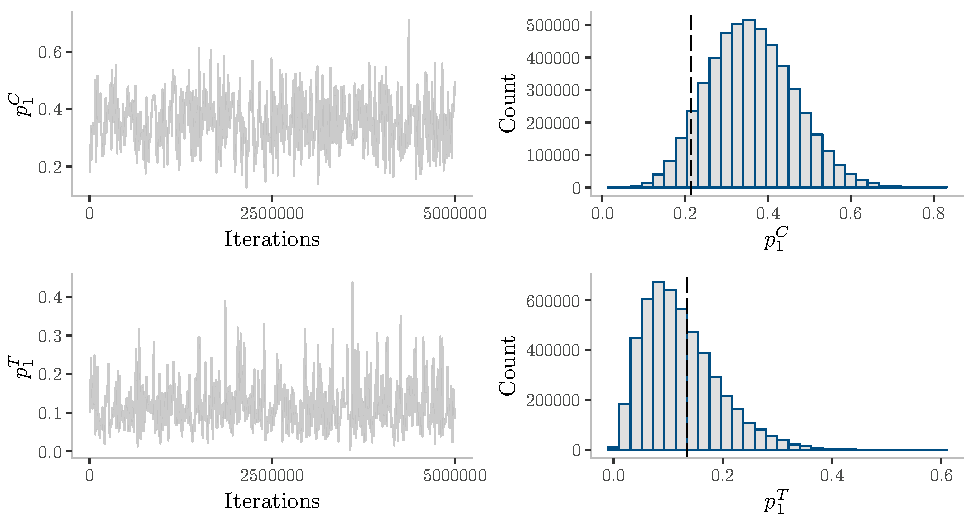
\includegraphics{thesis_files/figure-latex/unnamed-chunk-20-1.pdf}
\caption{\label{fig:unnamed-chunk-20}Submodel 1 posterior traceplots and
histograms for \(p_1^C\) and \(p_1^T\)}
\end{figure}

\begin{figure}
\centering
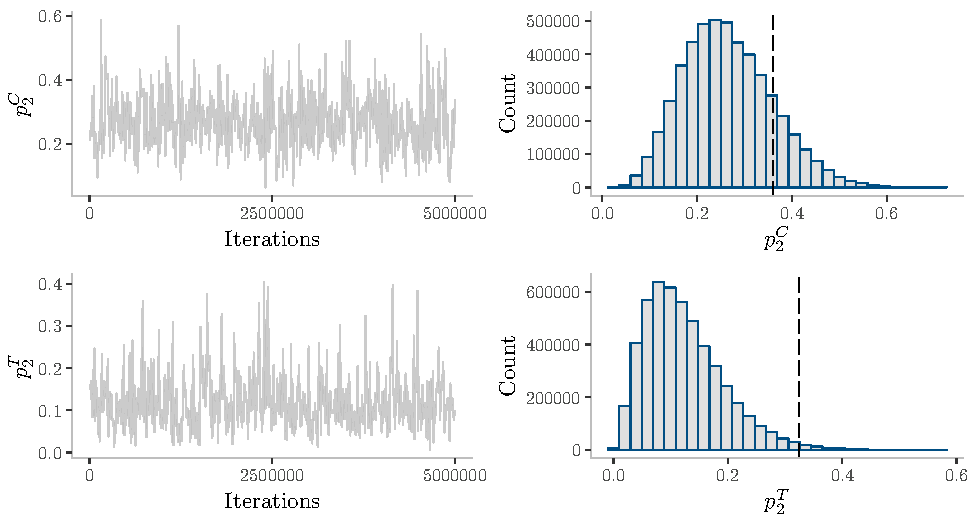
\includegraphics{thesis_files/figure-latex/unnamed-chunk-21-1.pdf}
\caption{\label{fig:unnamed-chunk-21}Submodel 1 posterior traceplots and
histograms for \(p_2^C\) and \(p_2^T\)}
\end{figure}

\begin{figure}
\centering
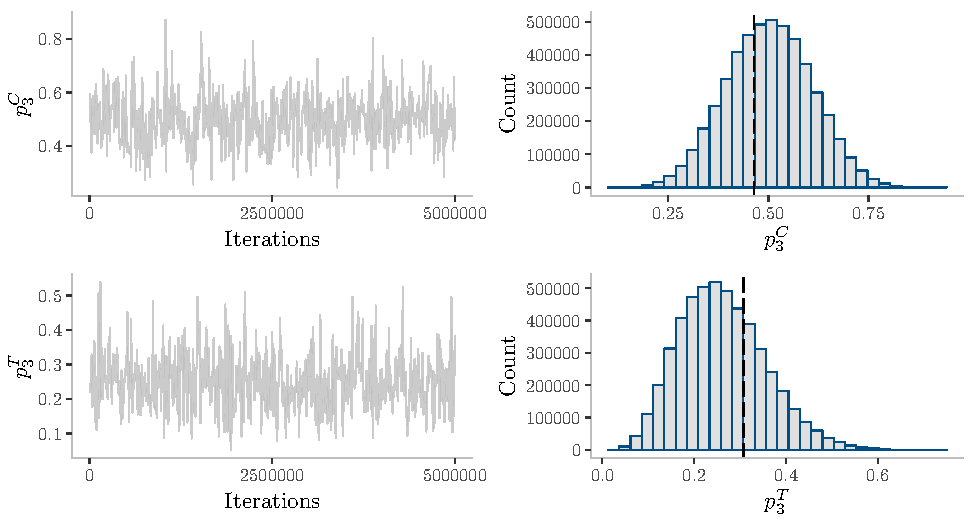
\includegraphics{thesis_files/figure-latex/unnamed-chunk-22-1.pdf}
\caption{\label{fig:unnamed-chunk-22}Submodel 1 posterior traceplots and
histograms for \(p_3^C\) and \(p_3^T\)}
\end{figure}

\begin{figure}
\centering
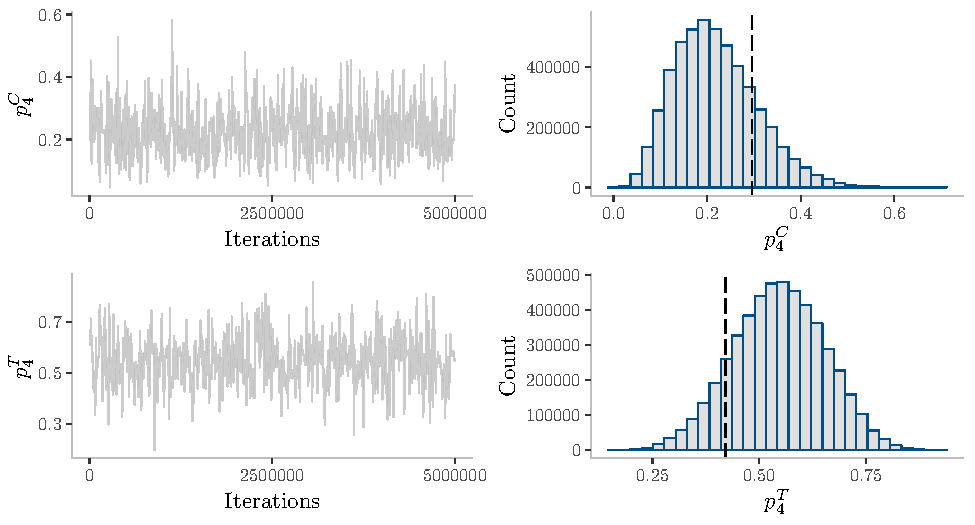
\includegraphics{thesis_files/figure-latex/unnamed-chunk-23-1.pdf}
\caption{\label{fig:unnamed-chunk-23}Submodel 1 posterior traceplots and
histograms for \(p_4^C\) and \(p_4^T\)}
\end{figure}

\begin{figure}
\centering
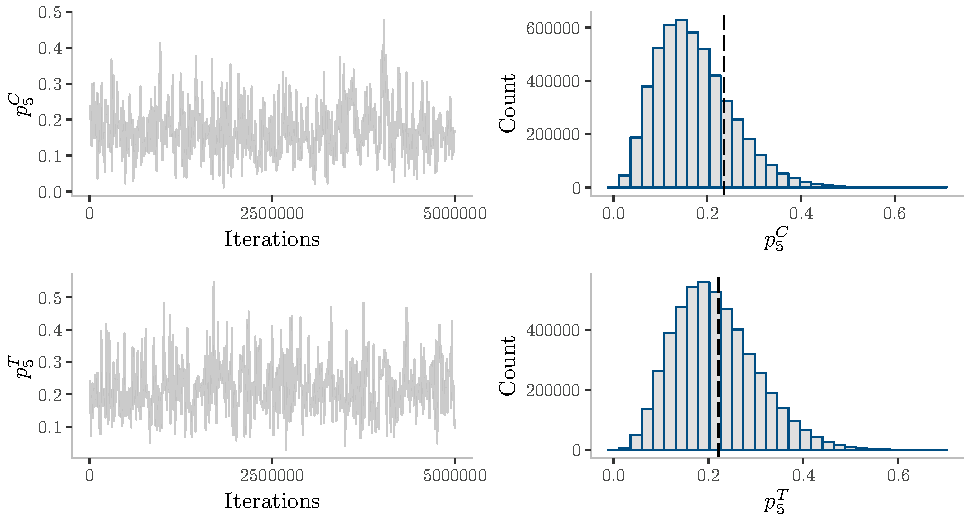
\includegraphics{thesis_files/figure-latex/unnamed-chunk-24-1.pdf}
\caption{\label{fig:unnamed-chunk-24}Submodel 1 posterior traceplots and
histograms for \(p_5^C\) and \(p_5^T\)}
\end{figure}

\newpage

\section{Melded model}\label{melded-model}

\begin{figure}
\centering
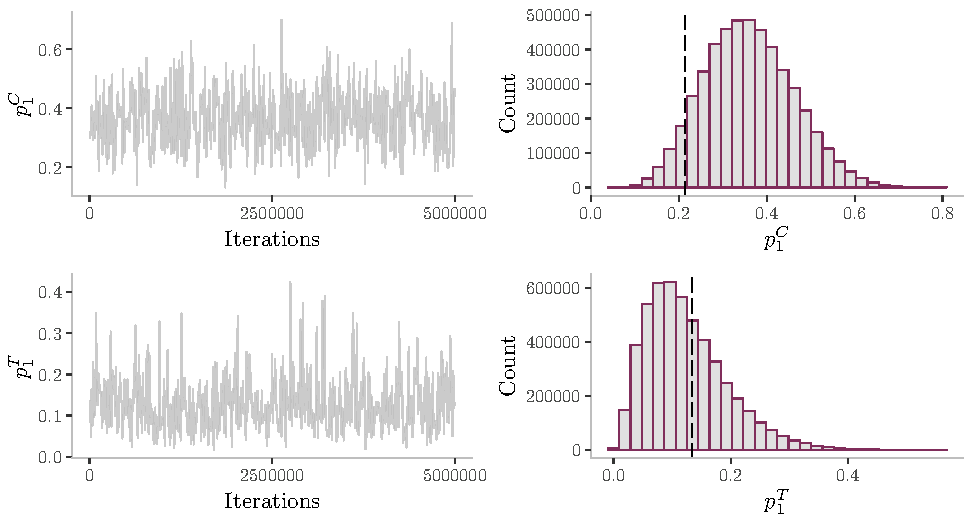
\includegraphics{thesis_files/figure-latex/unnamed-chunk-26-1.pdf}
\caption{\label{fig:unnamed-chunk-26}Melded model posterior traceplots and
histograms for \(p_1^C\) and \(p_1^T\)}
\end{figure}

\begin{figure}
\centering
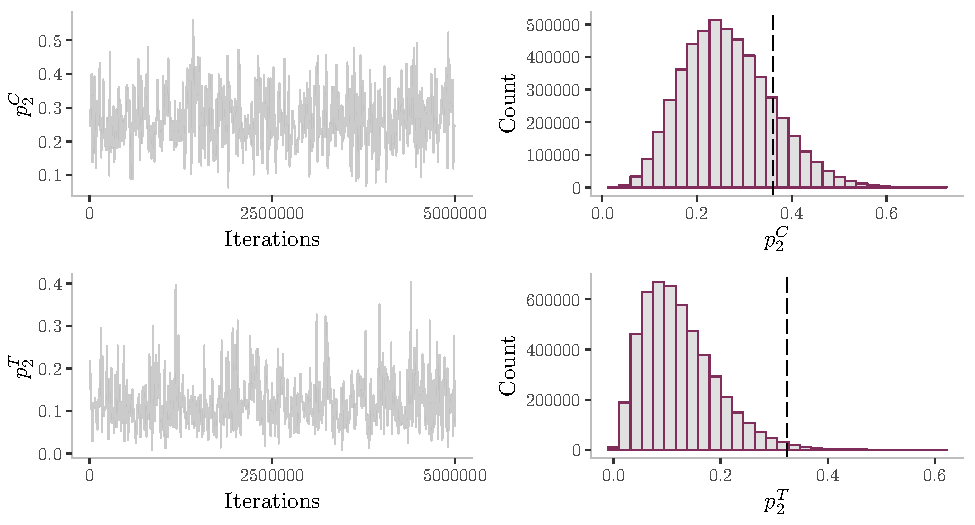
\includegraphics{thesis_files/figure-latex/unnamed-chunk-27-1.pdf}
\caption{\label{fig:unnamed-chunk-27}Melded model posterior traceplots and
histograms for \(p_2^C\) and \(p_2^T\)}
\end{figure}

\begin{figure}
\centering
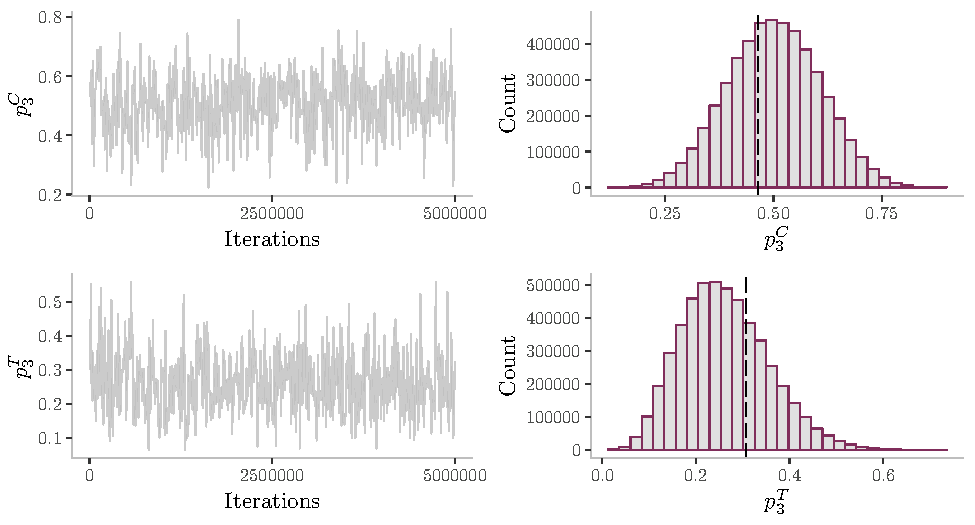
\includegraphics{thesis_files/figure-latex/unnamed-chunk-28-1.pdf}
\caption{\label{fig:unnamed-chunk-28}Melded model posterior traceplots and
histograms for \(p_3^C\) and \(p_3^T\)}
\end{figure}

\begin{figure}
\centering
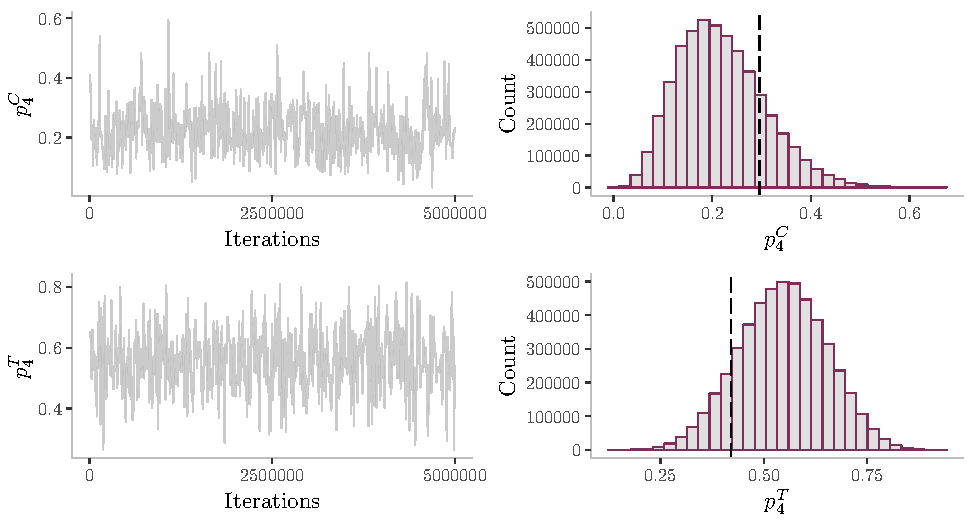
\includegraphics{thesis_files/figure-latex/unnamed-chunk-29-1.pdf}
\caption{\label{fig:unnamed-chunk-29}Melded model posterior traceplots and
histograms for \(p_4^C\) and \(p_4^T\)}
\end{figure}

\begin{figure}
\centering
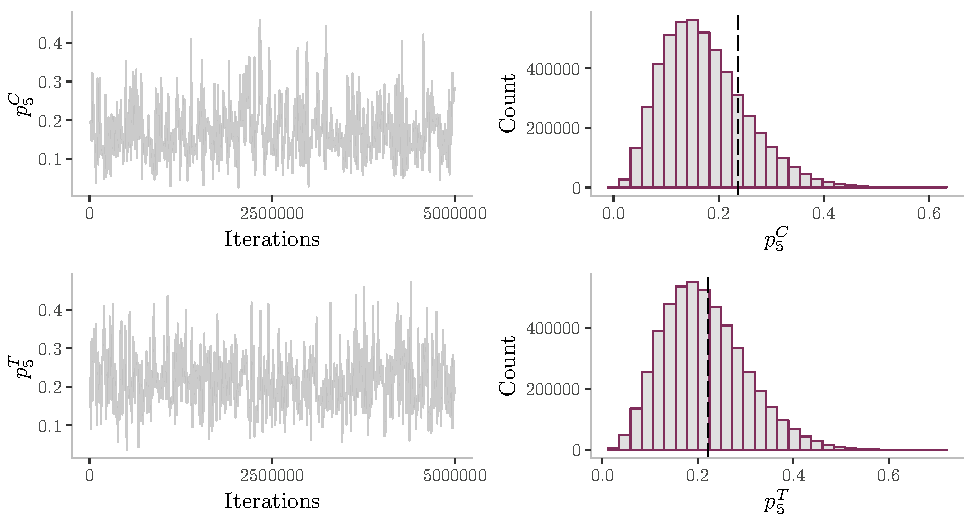
\includegraphics{thesis_files/figure-latex/unnamed-chunk-30-1.pdf}
\caption{\label{fig:unnamed-chunk-30}Melded model posterior traceplots and
histograms for \(p_5^C\) and \(p_5^T\)}
\end{figure}

\chapter*{Bibliography}\label{bibliography}
\addcontentsline{toc}{chapter}{Bibliography}

\hypertarget{refs}{}
\hypertarget{ref-ades2002markov}{}
Ades, AE, and S Cliffe. 2002. ``Markov Chain Monte Carlo Estimation of a
Multiparameter Decision Model: Consistency of Evidence and the Accurate
Assessment of Uncertainty.'' \emph{Medical Decision Making} 22 (4). Sage
Publications Sage CA: Thousand Oaks, CA: 359--71.

\hypertarget{ref-ashby2000evidence}{}
Ashby, Deborah, and Adrian FM Smith. 2000. ``Evidence-Based Medicine as
Bayesian Decision-Making.'' \emph{Statistics in Medicine} 19 (23). Wiley
Online Library: 3291--3305.

\hypertarget{ref-bishop2006pattern}{}
Bishop, Christopher M. 2006. \emph{Pattern Recognition and Machine
Learning}. Springer.

\hypertarget{ref-clemen1999combining}{}
Clemen, Robert T, and Robert L Winkler. 1999. ``Combining Probability
Distributions from Experts in Risk Analysis.'' \emph{Risk Analysis} 19
(2). Springer: 187--203.

\hypertarget{ref-dawid1993hyper}{}
Dawid, A Philip, and Steffen L Lauritzen. 1993. ``Hyper Markov Laws in
the Statistical Analysis of Decomposable Graphical Models.'' \emph{The
Annals of Statistics} 21 (3). Institute of Mathematical Statistics:
1272--1317.

\hypertarget{ref-mcmcse}{}
Flegal, James M., John Hughes, Dootika Vats, and Ning Dai. 2017.
\emph{mcmcse: Monte Carlo Standard Errors for MCMC}. Riverside, CA,
Denver, CO, Coventry, UK; Minneapolis, MN.

\hypertarget{ref-gelman1992inference}{}
Gelman, Andrew, Donald B Rubin, and others. 1992. ``Inference from
Iterative Simulation Using Multiple Sequences.'' \emph{Statistical
Science} 7 (4). Institute of Mathematical Statistics: 457--72.

\hypertarget{ref-geman1987stochastic}{}
Geman, Stuart, and Donald Geman. 1987. ``Stochastic relaxation, Gibbs
distributions, and the Bayesian restoration of images.'' In
\emph{Readings in Computer Vision}, 564--84. Elsevier.

\hypertarget{ref-gilks1995markov}{}
Gilks, Walter R, Sylvia Richardson, and David Spiegelhalter. 1995.
\emph{Markov Chain Monte Carlo in Practice}. Chapman; Hall/CRC.

\hypertarget{ref-goudie2019joining}{}
Goudie, Robert JB, Anne M Presanis, David Lunn, Daniela De Angelis, and
Lorenz Wernisch. 2019. ``Joining and Splitting Models with Markov
Melding.'' \emph{Bayesian Analysis} 14 (1). Europe PMC Funders: 81.

\hypertarget{ref-hastings1970monte}{}
Hastings, W Keith. 1970. ``Monte Carlo Sampling Methods Using Markov
Chains and Their Applications.'' Oxford University Press.

\hypertarget{ref-hickman2013multiple}{}
Hickman, Matthew, Daniela De Angelis, Hayley Jones, Ross Harris, Nicky
Welton, and AE Ades. 2013. ``Multiple Parameter Evidence Synthesis-a
Potential Solution for When Information on Drug Use and Harm Is in
Conflict.'' \emph{Addiction} 108 (9). Wiley Online Library: 1529--31.

\hypertarget{ref-hinton2002training}{}
Hinton, Geoffrey E. 2002. ``Training Products of Experts by Minimizing
Contrastive Divergence.'' \emph{Neural Computation} 14 (8). MIT Press:
1771--1800.

\hypertarget{ref-lindsten2017divide}{}
Lindsten, Fredrik, Adam M Johansen, Christian A Naesseth, Bonnie
Kirkpatrick, Thomas B Schön, JAD Aston, and Alexandre Bouchard-Côté.
2017. ``Divide-and-Conquer with Sequential Monte Carlo.'' \emph{Journal
of Computational and Graphical Statistics} 26 (2). Taylor \& Francis:
445--58.

\hypertarget{ref-lunn2013fully}{}
Lunn, David, Jessica Barrett, Michael Sweeting, and Simon Thompson.
2013. ``Fully Bayesian Hierarchical Modelling in Two Stages, with
Application to Meta-Analysis.'' \emph{Journal of the Royal Statistical
Society: Series C (Applied Statistics)} 62 (4). Wiley Online Library:
551--72.

\hypertarget{ref-metropolis1953equation}{}
Metropolis, Nicholas, Arianna W Rosenbluth, Marshall N Rosenbluth,
Augusta H Teller, and Edward Teller. 1953. ``Equation of State
Calculations by Fast Computing Machines.'' \emph{The Journal of Chemical
Physics} 21 (6). AIP: 1087--92.

\hypertarget{ref-muller1991generic}{}
Muller, Peter. 1991. ``A generic approach to posterior integration and
Gibbs sampling.'' \emph{Technical Report}, 91--09.

\hypertarget{ref-neal2006optimal}{}
Neal, Peter, and Gareth Roberts. 2006. ``Optimal scaling for partially
updating MCMC algorithms.'' \emph{The Annals of Applied Probability} 16
(2). Institute of Mathematical Statistics: 475--515.

\hypertarget{ref-o2006uncertain}{}
O'Hagan, Anthony, Caitlin E Buck, Alireza Daneshkhah, J Richard Eiser,
Paul H Garthwaite, David J Jenkinson, Jeremy E Oakley, and Tim Rakow.
2006. \emph{Uncertain Judgements: Eliciting Experts' Probabilities}.
John Wiley \& Sons.

\hypertarget{ref-poole2000inference}{}
Poole, David, and Adrian E Raftery. 2000. ``Inference for Deterministic
Simulation Models: The Bayesian Melding Approach.'' \emph{Journal of the
American Statistical Association} 95 (452). Taylor \& Francis Group:
1244--55.

\hypertarget{ref-presanis2014synthesising}{}
Presanis, Anne M, Richard G Pebody, Paul J Birrell, Brian DM Tom, Helen
K Green, Hayley Durnall, Douglas Fleming, Daniela De Angelis, and
others. 2014. ``Synthesising evidence to estimate pandemic (2009) A/H1N1
influenza severity in 2009-2011.'' \emph{The Annals of Applied
Statistics} 8 (4). Institute of Mathematical Statistics: 2378--2403.

\hypertarget{ref-phe}{}
Public Health England. 2008. ``HIV: Overall Prevalence.''
\url{https://www.gov.uk/guidance/hiv-overall-prevalence}.

\hypertarget{ref-r}{}
R Core Team. 2018. \emph{R: A Language and Environment for Statistical
Computing}. Vienna, Austria: R Foundation for Statistical Computing.
\url{https://www.R-project.org/}.

\hypertarget{ref-raftery1995inference}{}
Raftery, Adrian E, Geof H Givens, and Judith E Zeh. 1995. ``Inference
from a Deterministic Population Dynamics Model for Bowhead Whales.''
\emph{Journal of the American Statistical Association} 90 (430). Taylor
\& Francis Group: 402--16.

\hypertarget{ref-robert2013monte}{}
Robert, Christian, and George Casella. 2013. \emph{Monte Carlo
Statistical Methods}. Springer Science \& Business Media.

\hypertarget{ref-roberts1997weak}{}
Roberts, Gareth, Andrew Gelman, and Walter R Gilks. 1997. ``Weak
Convergence and Optimal Scaling of Random Walk Metropolis Algorithms.''
\emph{The Annals of Applied Probability} 7 (1). Institute of
Mathematical Statistics: 110--20.

\hypertarget{ref-royal}{}
Royal Society, Academy of Medical Sciences. 2018. ``Evidence Synthesis
for Policy: A Statement of Principles.''
\url{https://royalsociety.org/-/media/policy/projects/evidence-synthesis/evidence-synthesis-statement-principles.pdf}.

\hypertarget{ref-schweder1996bayesian}{}
Schweder, Tore, and Nils Lid Hjort. 1996. ``Bayesian Synthesis or
Likelihood Synthesis - What Does Borel's Paradox Say?'' \emph{Preprint
Series. Statistical Research Report}. Matematisk Institutt,
Universitetet i Oslo.

\hypertarget{ref-smith1995bayesian}{}
Smith, Teresa, David J Spiegelhalter, and Andrew Thomas. 1995.
``Bayesian Approaches to Random-Effects Meta-Analysis: A Comparative
Study.'' \emph{Statistics in Medicine} 14 (24). Wiley Online Library:
2685--99.

\hypertarget{ref-vats2015multivariate}{}
Vats, Dootika, James M Flegal, and Galin L Jones. 2015. ``Multivariate
Output Analysis for Markov Chain Monte Carlo.'' \emph{arXiv Preprint
arXiv:1512.07713}.

\hypertarget{ref-welton2012evidence}{}
Welton, Nicky, Alexander J Sutton, Nicola Cooper, Keith R Abrams, and AE
Ades. 2012. \emph{Evidence Synthesis for Decision Making in Healthcare}.
Vol. 132. John Wiley \& Sons.

\hypertarget{ref-ggplot2}{}
Wickham, Hadley. 2016. \emph{ggplot2: Elegant Graphics for Data
Analysis}. Springer-Verlag New York.
\url{https://ggplot2.tidyverse.org}.

\hypertarget{ref-wolpert1995inference}{}
Wolpert, Robert L. 1995. ``Inference from a Deterministic Population
Dynamics Model for Bowhead Whales: Comment.'' \emph{Journal of the
American Statistical Association} 90 (430). JSTOR: 426--27.

\hypertarget{ref-bookdown}{}
Xie, Yihui. 2016. \emph{bookdown: Authoring Books and Technical
Documents with R Markdown}. Boca Raton, Florida: Chapman; Hall/CRC.
\url{https://github.com/rstudio/bookdown}.

\end{document}
